\subsection{Численные эксперименты для первой задачи}

Рассматривается задача (\ref{nonsmooth:1}).
Зафиксируем выбранные опытным путём
$$ \tau = 10^{-3}, \; h = 10^{-2}, \; \varepsilon = 10^{-2}$$

Будем рассматривать зависимости 
$ p(\rho) = C \rho $ и $p(\rho) = \rho^{\gamma}$
и внешние параметры 
$$ (C, \mu) \in \{1, 10\} \times \{0.1, 0.01\}, \; \gamma = 1.4$$


\subsubsection{Время стабилизации и ошибки решения}
Далее приведена таблицы значений $\left\|V^{n}\right\|_C$. 

В каждой ячейке таблицы приведены значения для сеток
$ \bar Q_{\tau, h} $, $ \bar Q_{\tau, h/2} $, 
$ \bar Q_{\tau/2, h} $, $ \bar Q_{\tau/2, h/2} $ соответственно.

\begin{table}[H]
\centering
\begin{tabular}{|c|c|c|c|c|c|}
\hline
 & $N_{0} \tau$  & $n=N_{0}/4$ & $n=N_{0} / 2$ & $n=3N_{0} / 4$ & $n=N_{0}$ \\
\hline
 & \texttt{64.1290} & \texttt{1.396156e-01} & \texttt{9.770485e-02} & \texttt{4.554561e-02} & \texttt{9.990253e-03} \\
$C = 1$
 & \texttt{64.1300} & \texttt{1.401766e-01} & \texttt{9.804964e-02} & \texttt{4.562840e-02} & \texttt{9.990907e-03} \\
$\mu = 0.1$
 & \texttt{64.1305} & \texttt{1.402810e-01} & \texttt{9.811721e-02} & \texttt{4.561001e-02} & \texttt{9.990522e-03} \\
 & \texttt{64.1315} & \texttt{1.408454e-01} & \texttt{9.847310e-02} & \texttt{4.569729e-02} & \texttt{9.994465e-03} \\
\hline
 & \texttt{77.0350} & \texttt{2.906708e-01} & \texttt{1.327069e-01} & \texttt{5.033752e-02} & \texttt{9.937961e-03} \\
$C = 10$
 & \texttt{77.0340} & \texttt{2.913508e-01} & \texttt{1.328551e-01} & \texttt{5.048223e-02} & \texttt{9.999980e-03} \\
$\mu = 0.1$
 & \texttt{80.1815} & \texttt{1.210648e-01} & \texttt{1.289557e-01} & \texttt{7.039494e-02} & \texttt{9.992452e-03} \\
 & \texttt{81.7540} & \texttt{2.056498e-01} & \texttt{7.876163e-02} & \texttt{3.097946e-02} & \texttt{9.978467e-03} \\
\hline
 & \texttt{69.5600} & \texttt{1.563148e-01} & \texttt{9.869631e-02} & \texttt{4.241056e-02} & \texttt{9.980259e-03} \\
$\gamma = 1.4$
 & \texttt{69.5550} & \texttt{1.568927e-01} & \texttt{9.898179e-02} & \texttt{4.248563e-02} & \texttt{9.977743e-03} \\
$\mu = 0.1$
 & \texttt{69.5560} & \texttt{1.573937e-01} & \texttt{9.917836e-02} & \texttt{4.251199e-02} & \texttt{9.995456e-03} \\
 & \texttt{69.5510} & \texttt{1.579854e-01} & \texttt{9.944954e-02} & \texttt{4.258724e-02} & \texttt{9.992397e-03} \\
\hline
 & \texttt{278.2240} & \texttt{8.603387e-02} & \texttt{3.767792e-02} & \texttt{1.924198e-02} & \texttt{9.997962e-03} \\
$C = 1$
 & \texttt{278.2280} & \texttt{8.596664e-02} & \texttt{3.763429e-02} & \texttt{1.922858e-02} & \texttt{9.999739e-03} \\
$\mu = 0.01$
 & \texttt{288.1590} & \texttt{7.650990e-02} & \texttt{3.666142e-02} & \texttt{3.359777e-02} & \texttt{9.996764e-03} \\
 & \texttt{288.1630} & \texttt{7.675698e-02} & \texttt{3.661180e-02} & \texttt{3.361363e-02} & \texttt{9.999931e-03} \\
\hline
 & \texttt{216.0880} & \texttt{1.588704e-01} & \texttt{6.030228e-02} & \texttt{2.660252e-02} & \texttt{9.988689e-03} \\ 
$C = 10$
 & \texttt{216.0890} & \texttt{1.588565e-01} & \texttt{6.043748e-02} & \texttt{2.667736e-02} & \texttt{9.994787e-03} \\
$\mu = 0.01$
 & \texttt{247.6790} & \texttt{1.418862e-01} & \texttt{5.378805e-02} & \texttt{2.447350e-02} & \texttt{9.995949e-03} \\
 & \texttt{247.6810} & \texttt{1.420525e-01} & \texttt{5.388815e-02} & \texttt{2.450650e-02} & \texttt{9.998647e-03} \\
\hline
 & \texttt{247.5020} & \texttt{8.835711e-02} & \texttt{3.691059e-02} & \texttt{1.870417e-02} & \texttt{9.996049e-03} \\
$\gamma = 1.4$
 & \texttt{247.4830} & \texttt{8.819201e-02} & \texttt{3.684642e-02} & \texttt{1.869037e-02} & \texttt{9.997412e-03} \\
$\mu = 0.01$
 & \texttt{251.5215} & \texttt{1.113215e-01} & \texttt{4.525027e-02} & \texttt{2.172460e-02} & \texttt{9.997047e-03} \\
 & \texttt{251.5025} & \texttt{1.114972e-01} & \texttt{4.531320e-02} & \texttt{2.174818e-02} & \texttt{9.996424e-03} \\
\hline
\end{tabular}
\caption{Ошибки для скорости при $\tau = 10^{-3}$, $h = 10^{-2}$.}
\end{table}

\newpage
\begin{figure}[H]
\center{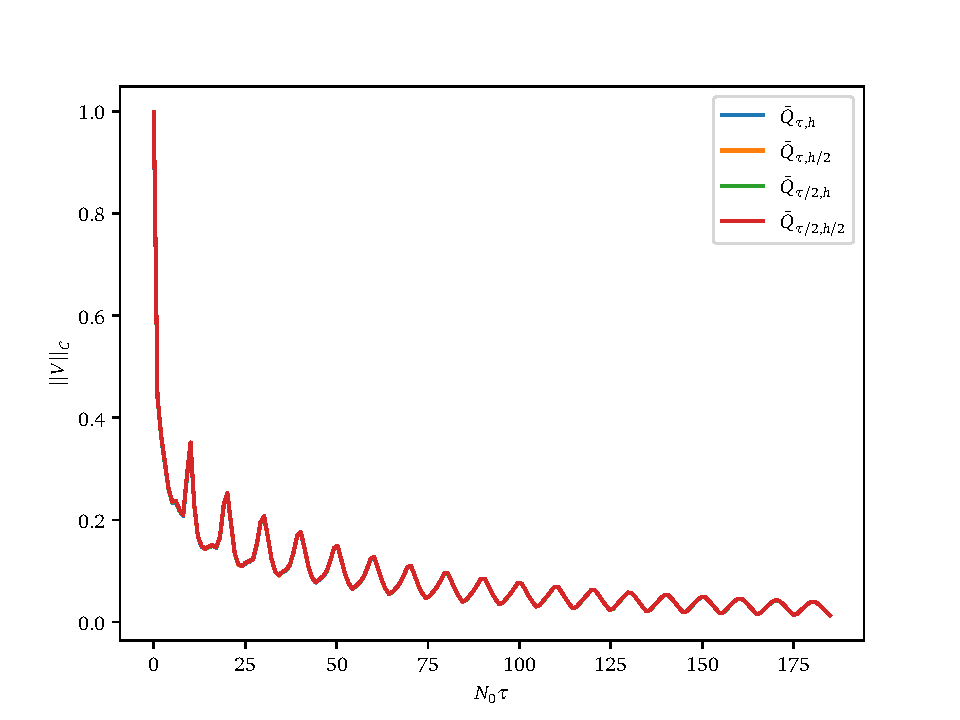
\includegraphics[scale=0.9]{pics_1d/norm_V_4_1_1_0.1.pdf}}
\caption{График $\left\| V \right\|_C$ при $C = 1$, $\gamma = 1$ и~$\mu = 0.1$.}
\end{figure}

\begin{figure}[H]
\center{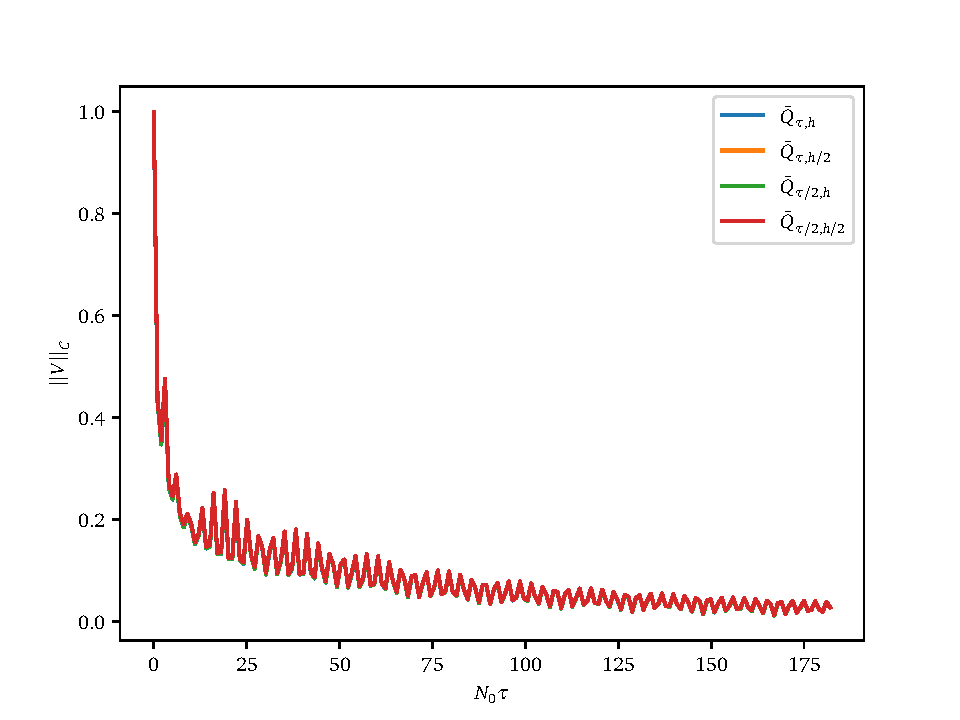
\includegraphics[scale=0.9]{pics_1d/norm_V_4_10_1_0.1.pdf}}
\caption{График $\left\| V \right\|_C$ при $C = 10$, $\gamma = 1$ и~$\mu = 0.1$.}
\end{figure}

\begin{figure}[H]
\center{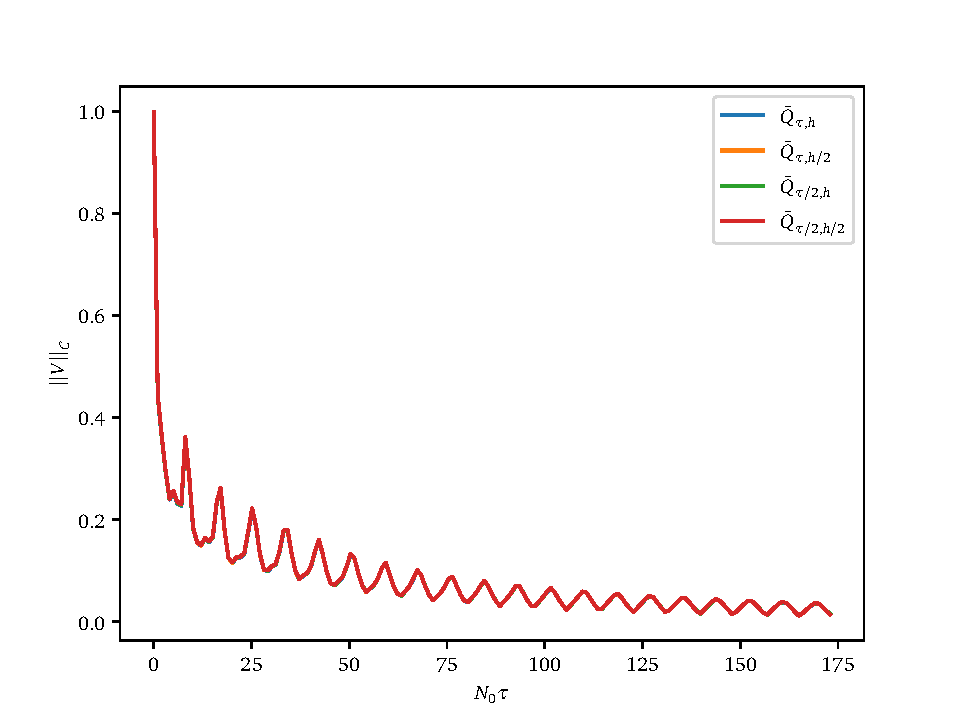
\includegraphics[scale=0.9]{pics_1d/norm_V_4_1_1.4_0.1.pdf}}
\caption{График $\left\| V \right\|_C$ при $C = 1$, $\gamma = 1.4$ и~$\mu = 0.1$.}
\end{figure}

\begin{figure}[H]
\center{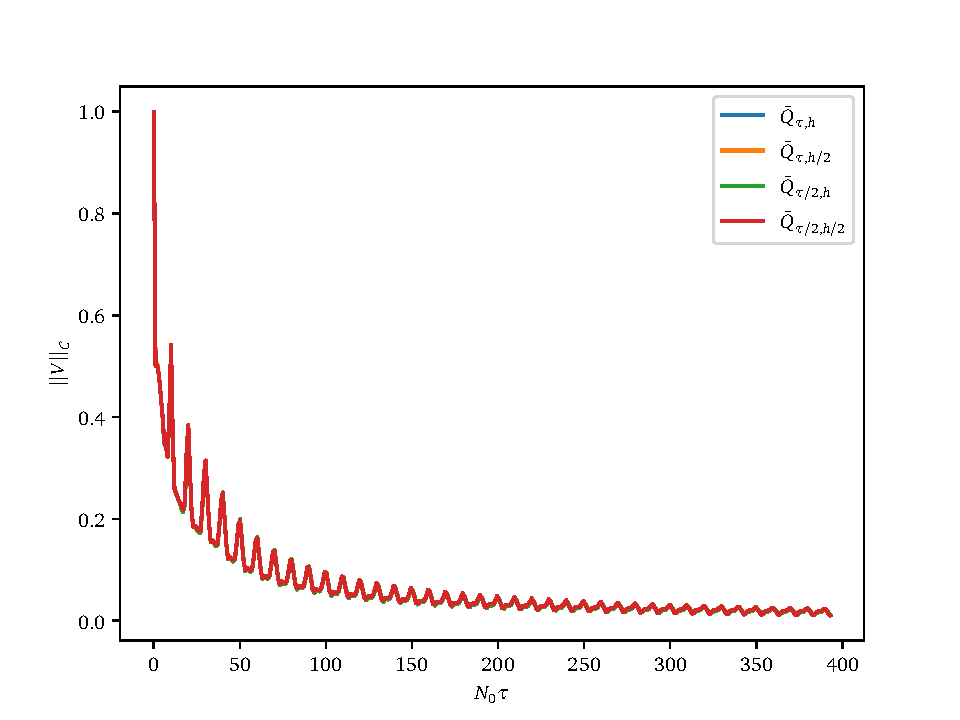
\includegraphics[scale=0.9]{pics_1d/norm_V_4_1_1_0.01.pdf}}
\caption{График $\left\| V \right\|_C$ при $C = 1$, $\gamma = 1$ и~$\mu = 0.01$.}
\end{figure}

\begin{figure}[H]
\center{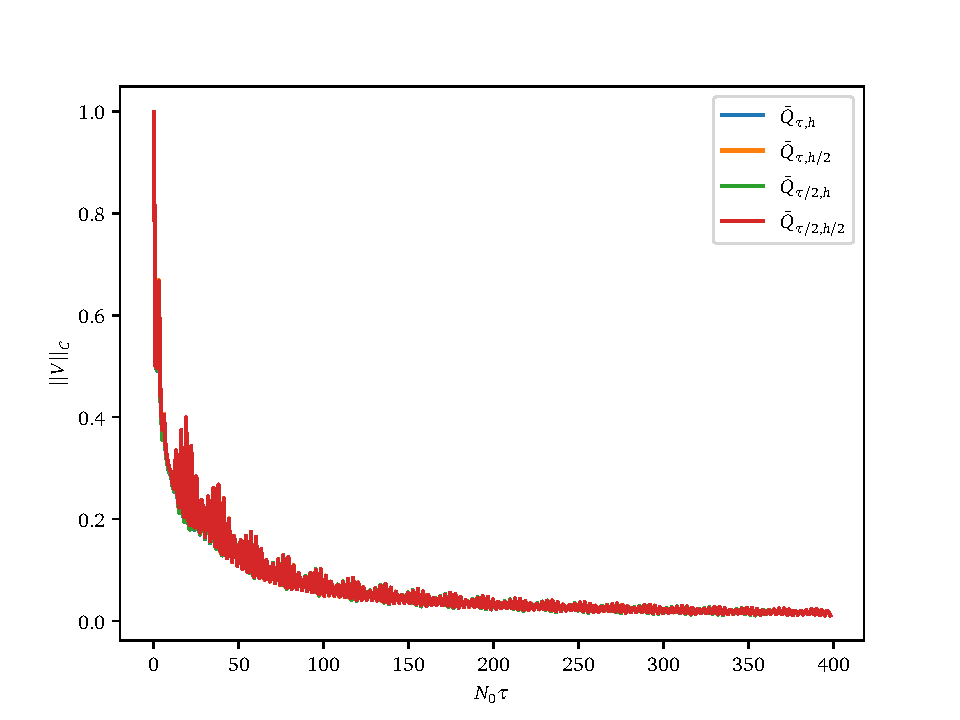
\includegraphics[scale=0.9]{pics_1d/norm_V_4_10_1_0.01.pdf}}
\caption{График $\left\| V \right\|_C$ при $C = 10$, $\gamma = 1$ и~$\mu = 0.01$.}
\end{figure}

\begin{figure}[H]
\center{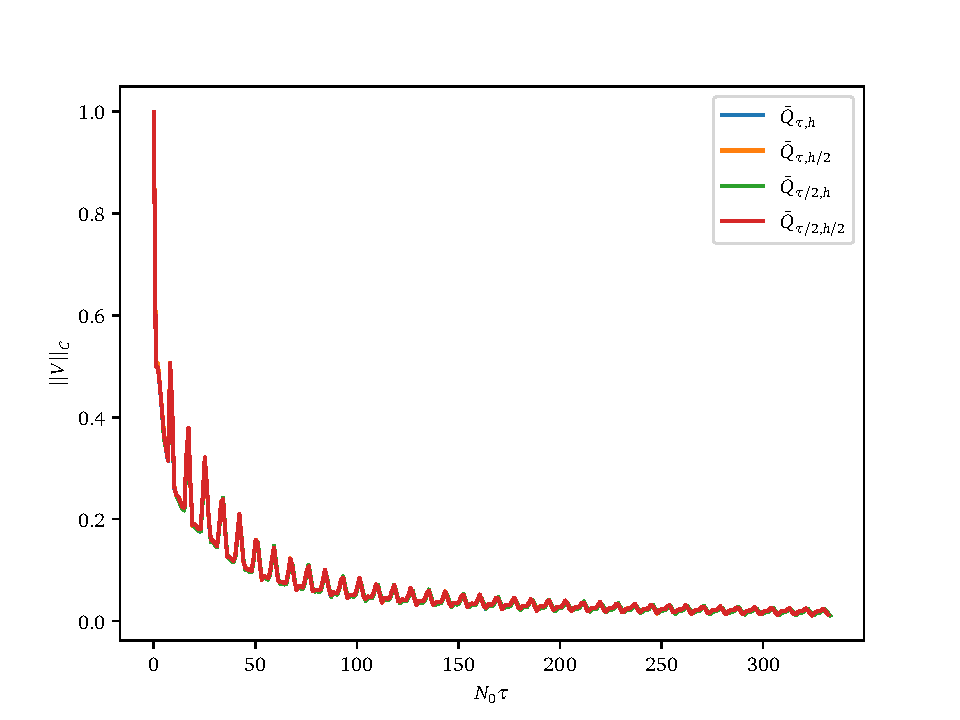
\includegraphics[scale=0.9]{pics_1d/norm_V_4_1_1.4_0.01.pdf}}
\caption{График $\left\| V \right\|_C$ при $C = 1$, $\gamma = 1.4$ и~$\mu = 0.01$.}
\end{figure}



\subsubsection{Консервативность решения}
Далее приведена таблица значений $\Delta_{m}(n)$. 

В каждой ячейке таблицы приведены значения для сеток
$ \bar Q_{\tau, h} $, $ \bar Q_{\tau, h/2} $, 
$ \bar Q_{\tau/2, h} $, $ \bar Q_{\tau/2, h/2} $ соответственно.

\begin{table}[H]
\centering
\begin{tabular}{|c|c|c|c|c|c|}
\hline
 & $n=N_{0}/5$ & $n=2N_{0}/5$ & $n=3N_{0}/5$ & $n=4N_{0}/5$ & $n=N_{0}$ \\
\hline
 & \texttt{-1.576194e-04} & \texttt{-1.981958e-04} & \texttt{-3.166168e-04} & \texttt{-3.012438e-04} & \texttt{-2.252491e-04} \\
$C = 1$
 & \texttt{-2.567727e-04} & \texttt{-2.970707e-04} & \texttt{-3.637339e-04} & \texttt{-3.604177e-04} & \texttt{-3.245736e-04} \\
$\mu = 0.1$
 & \texttt{1.546621e-05}  & \texttt{-7.496624e-06} & \texttt{-1.188958e-04} & \texttt{-9.883572e-05} & \texttt{-2.044277e-05} \\
 & \texttt{-7.924696e-05} & \texttt{-1.009926e-04} & \texttt{-1.605399e-04} & \texttt{-1.526765e-04} & \texttt{-1.145356e-04} \\
\hline
 & \texttt{-3.228625e-03} & \texttt{-3.368588e-03} & \texttt{-3.396079e-03} & \texttt{-3.401341e-03} & \texttt{-3.404017e-03} \\
$C = 10$
 & \texttt{-3.278029e-03} & \texttt{-3.443403e-03} & \texttt{-3.482686e-03} & \texttt{-3.494137e-03} & \texttt{-3.499076e-03} \\
$\mu = 0.1$
 & \texttt{-1.736748e-03} & \texttt{-1.721632e-03} & \texttt{-1.740789e-03} & \texttt{-1.760467e-03} & \texttt{-1.773013e-03} \\
 & \texttt{-1.685181e-03} & \texttt{-1.802108e-03} & \texttt{-1.845356e-03} & \texttt{-1.862697e-03} & \texttt{-1.870293e-03} \\
\hline
 & \texttt{-4.632917e-04} & \texttt{-3.701415e-04} & \texttt{-5.665389e-04} & \texttt{-5.237228e-04} & \texttt{-4.781895e-04} \\
$\gamma = 1.4$
 & \texttt{-5.208406e-04} & \texttt{-4.986245e-04} & \texttt{-6.073323e-04} & \texttt{-5.901398e-04} & \texttt{-5.696901e-04} \\
$\mu = 0.1$
 & \texttt{-1.845740e-04} & \texttt{-6.699655e-05} & \texttt{-2.542901e-04} & \texttt{-2.071144e-04} & \texttt{-1.588117e-04} \\
 & \texttt{-2.365174e-04} & \texttt{-1.900707e-04} & \texttt{-2.891894e-04} & \texttt{-2.677119e-04} & \texttt{-2.447111e-04} \\
\hline
 & \texttt{-3.130581e-03} & \texttt{-3.270885e-03} & \texttt{-3.420731e-03} & \texttt{-3.399867e-03} & \texttt{-3.454908e-03} \\
$C = 1$
 & \texttt{-3.189063e-03} & \texttt{-3.367047e-03} & \texttt{-3.471238e-03} & \texttt{-3.471312e-03} & \texttt{-3.503626e-03} \\
$\mu = 0.01$
 & \texttt{-1.704495e-03} & \texttt{-1.752921e-03} & \texttt{-1.757478e-03} & \texttt{-1.815081e-03} & \texttt{-1.821601e-03} \\
 & \texttt{-1.730221e-03} & \texttt{-1.811384e-03} & \texttt{-1.828262e-03} & \texttt{-1.862207e-03} & \texttt{-1.867927e-03} \\
\hline
 & \texttt{-1.491760e-02} & \texttt{-1.518193e-02} & \texttt{-1.527227e-02} & \texttt{-1.527551e-02} & \texttt{-1.527354e-02} \\
$C = 10$
 & \texttt{-1.498850e-02} & \texttt{-1.526724e-02} & \texttt{-1.533916e-02} & \texttt{-1.534953e-02} & \texttt{-1.535239e-02} \\
$\mu = 0.01$
 & \texttt{-1.106924e-02} & \texttt{-1.120334e-02} & \texttt{-1.126469e-02} & \texttt{-1.126088e-02} & \texttt{-1.125641e-02} \\
 & \texttt{-1.102762e-02} & \texttt{-1.117432e-02} & \texttt{-1.121923e-02} & \texttt{-1.122199e-02} & \texttt{-1.122184e-02} \\
\hline
 & \texttt{-4.883364e-03} & \texttt{-5.077536e-03} & \texttt{-5.111989e-03} & \texttt{-5.120784e-03} & \texttt{-5.123262e-03} \\
$\gamma = 1.4$
 & \texttt{-4.874091e-03} & \texttt{-5.088341e-03} & \texttt{-5.131940e-03} & \texttt{-5.145525e-03} & \texttt{-5.150902e-03} \\
$\mu = 0.01$
 & \texttt{-2.743725e-03} & \texttt{-2.725259e-03} & \texttt{-2.779172e-03} & \texttt{-2.801832e-03} & \texttt{-2.813967e-03} \\
 & \texttt{-2.734016e-03} & \texttt{-2.788550e-03} & \texttt{-2.829544e-03} & \texttt{-2.845748e-03} & \texttt{-2.854010e-03} \\
\hline
\end{tabular}
\caption{Разность масс при $\tau = 10^{-3}$, $h = 10^{-2}$.}
\end{table}

 




\newpage
\begin{figure}[H]
\center{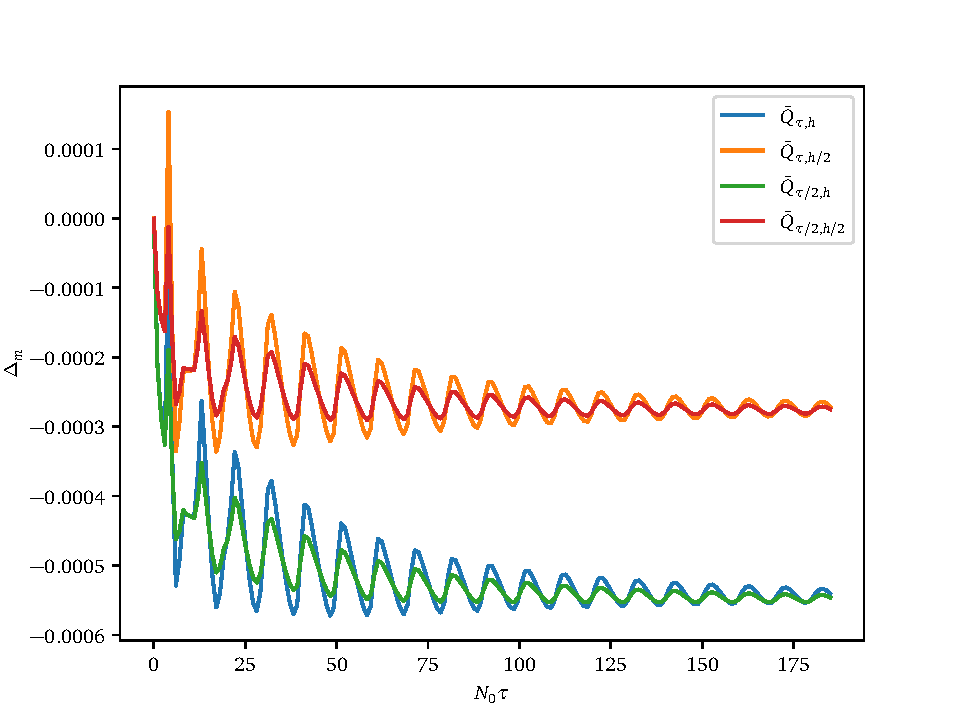
\includegraphics[scale=0.9]{pics_1d/diff_mass_4_1_1_0.1.pdf}}
\caption{График $\Delta_{m}$ при $C = 1$, $\gamma = 1$ и~$\mu = 0.1$.}
\end{figure}

\begin{figure}[H]
\center{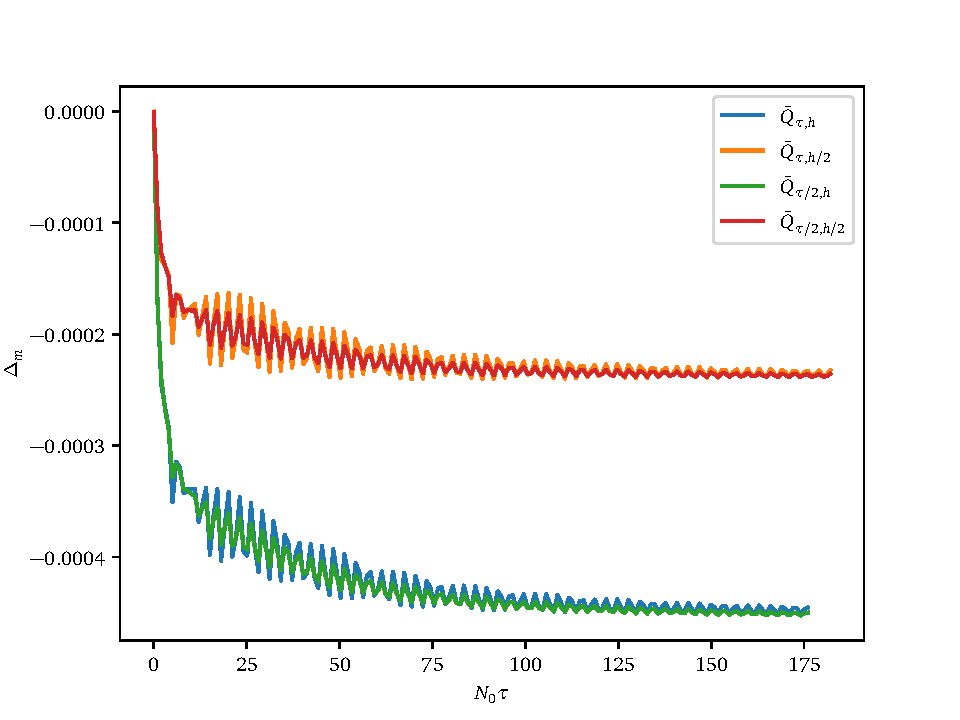
\includegraphics[scale=0.9]{pics_1d/diff_mass_4_10_1_0.1.pdf}}
\caption{График $\Delta_{m}$ при $C = 10$, $\gamma = 1$ и~$\mu = 0.1$.}
\end{figure}

\begin{figure}[H]
\center{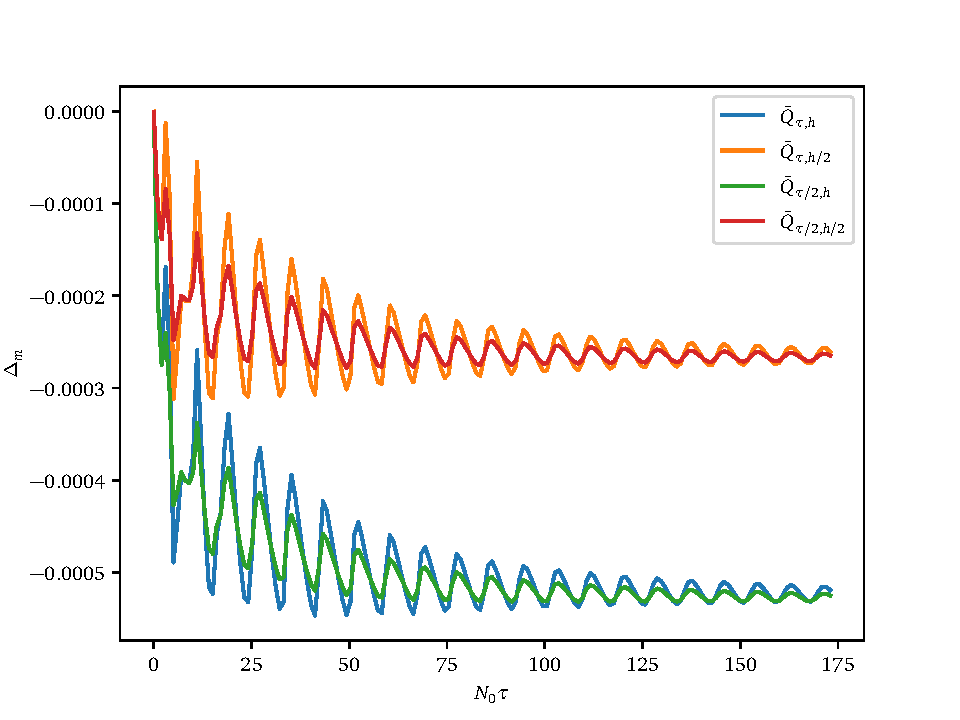
\includegraphics[scale=0.9]{pics_1d/diff_mass_4_1_1.4_0.1.pdf}}
\caption{График $\Delta_{m}$ при $C = 1$, $\gamma = 1.4$ и~$\mu = 0.1$.}
\end{figure}

\begin{figure}[H]
\center{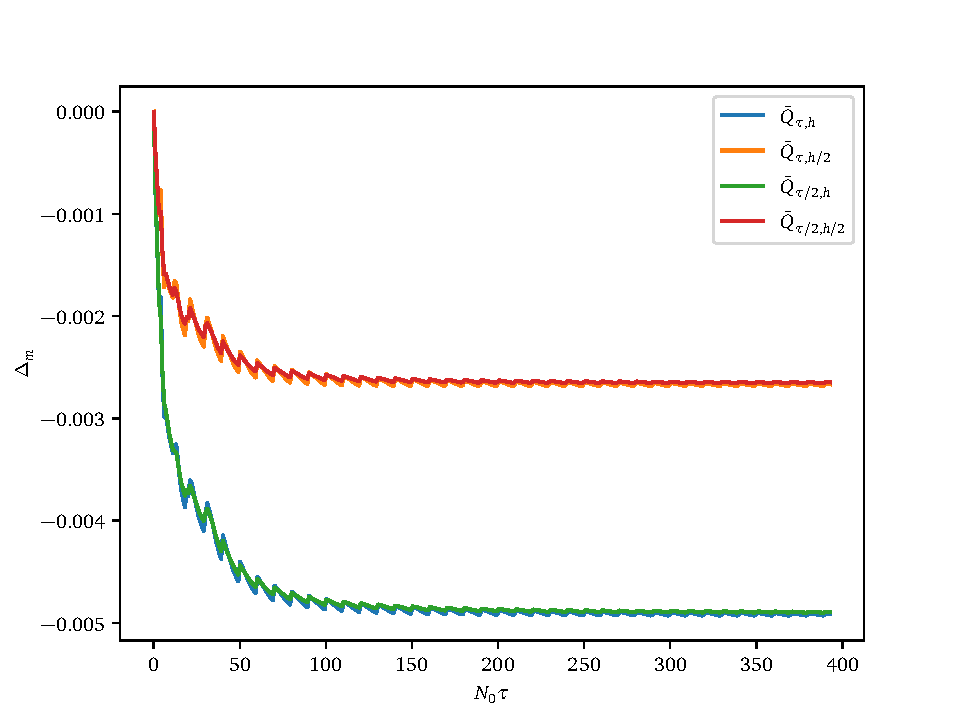
\includegraphics[scale=0.9]{pics_1d/diff_mass_4_1_1_0.01.pdf}}
\caption{График $\Delta_{m}$ при $C = 1$, $\gamma = 1$ и~$\mu = 0.01$.}
\end{figure}

\begin{figure}[H]
\center{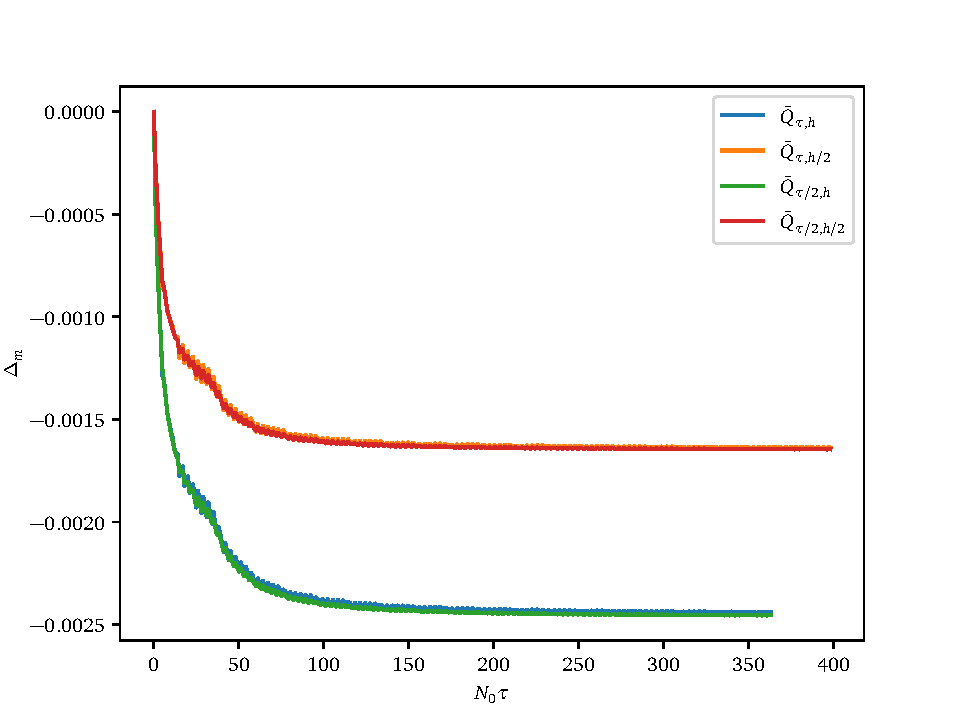
\includegraphics[scale=0.9]{pics_1d/diff_mass_4_10_1_0.01.pdf}}
\caption{График $\Delta_{m}$ при $C = 10$, $\gamma = 1$ и~$\mu = 0.01$.}
\end{figure}

\begin{figure}[H]
\center{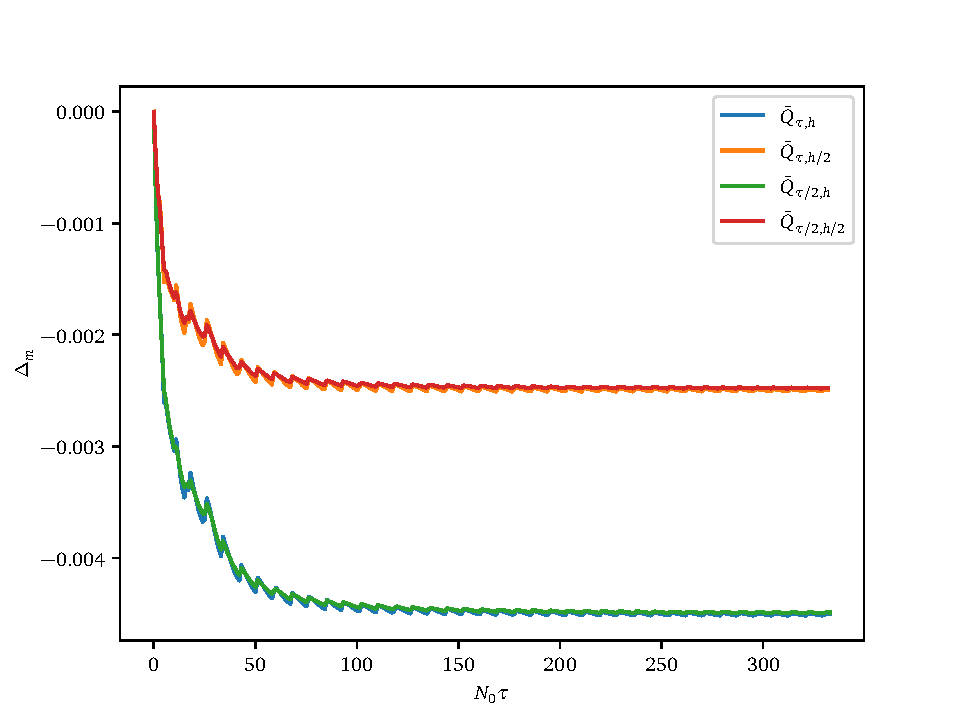
\includegraphics[scale=0.9]{pics_1d/diff_mass_4_1_1.4_0.01.pdf}}
\caption{График $\Delta_{m}$ при $C = 1$, $\gamma = 1.4$ и~$\mu = 0.01$.}
\end{figure}



\subsubsection{Динамика процесса решения}
Рассмотрим $C = 1, \; \gamma = 1, \; \mu = 0.1$.
Далее приведены срезы графиков $V$ и $G$ (динамика процесса) в разные моменты времени.
\begin{figure}[H]
\center{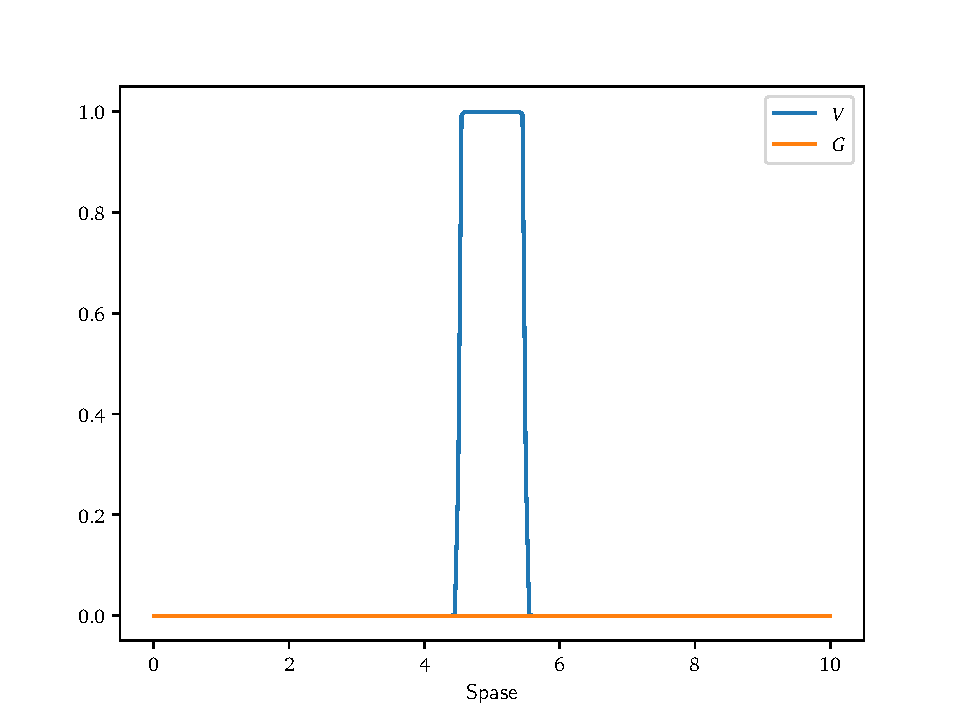
\includegraphics[scale=0.85]{pics_1d_cut/cut_4_1_1_0.1_0.pdf}}
\caption{Срез для $t=0$.}
\end{figure}

\begin{figure}[H]
\center{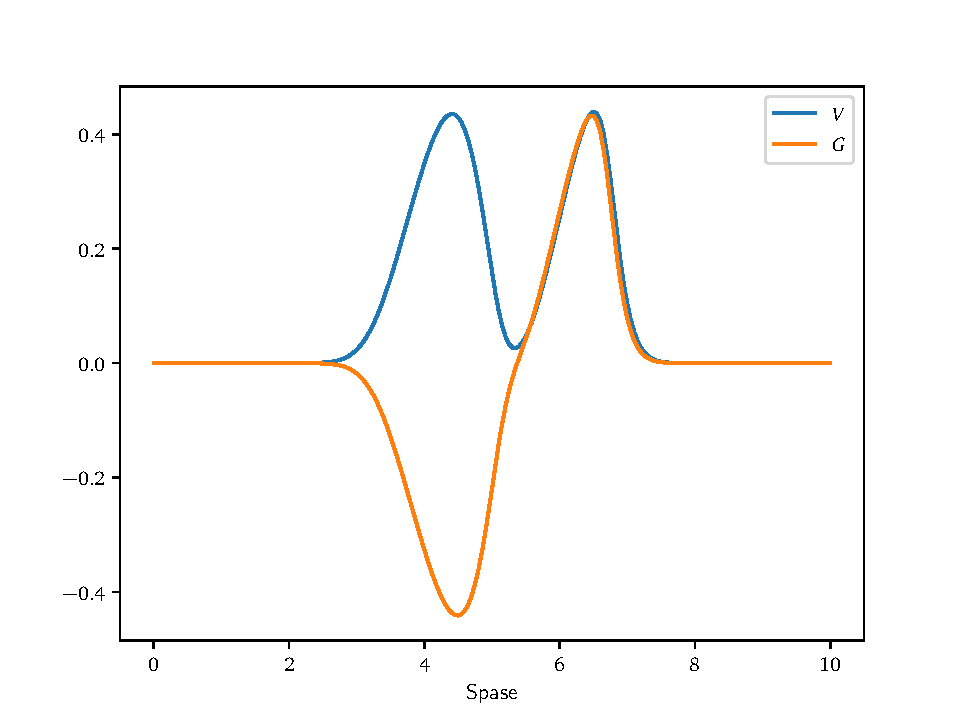
\includegraphics[scale=0.85]{pics_1d_cut/cut_4_1_1_0.1_1.pdf}}
\caption{Срез для $t=1$.}
\end{figure}

\begin{figure}[H]
\center{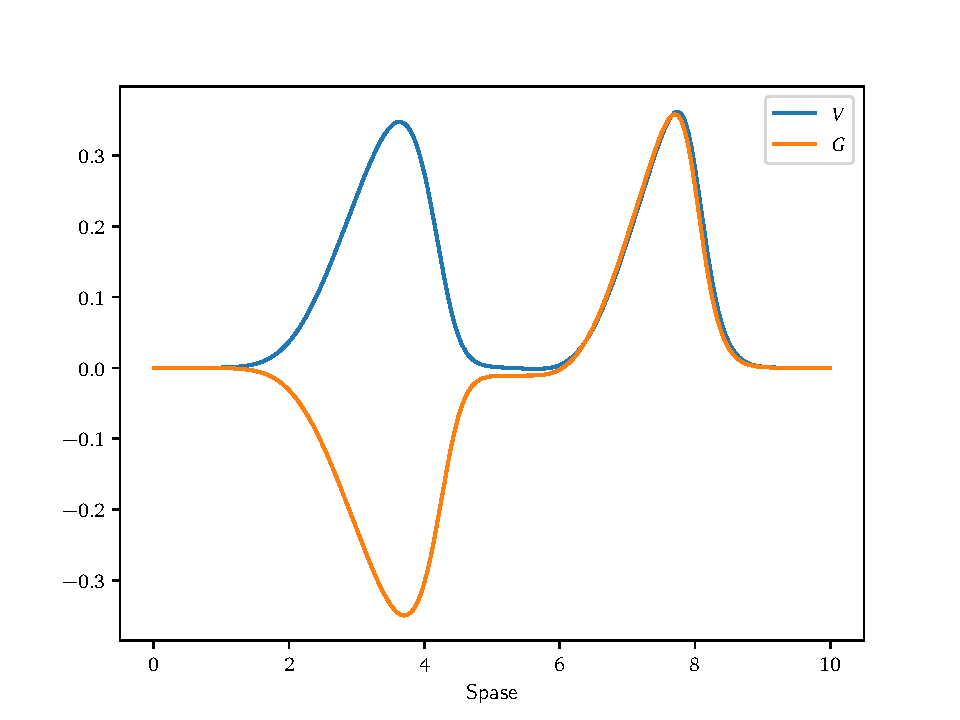
\includegraphics[scale=0.9]{pics_1d_cut/cut_4_1_1_0.1_2.pdf}}
\caption{Срез для $t=2$.}
\end{figure}

\begin{figure}[H]
\center{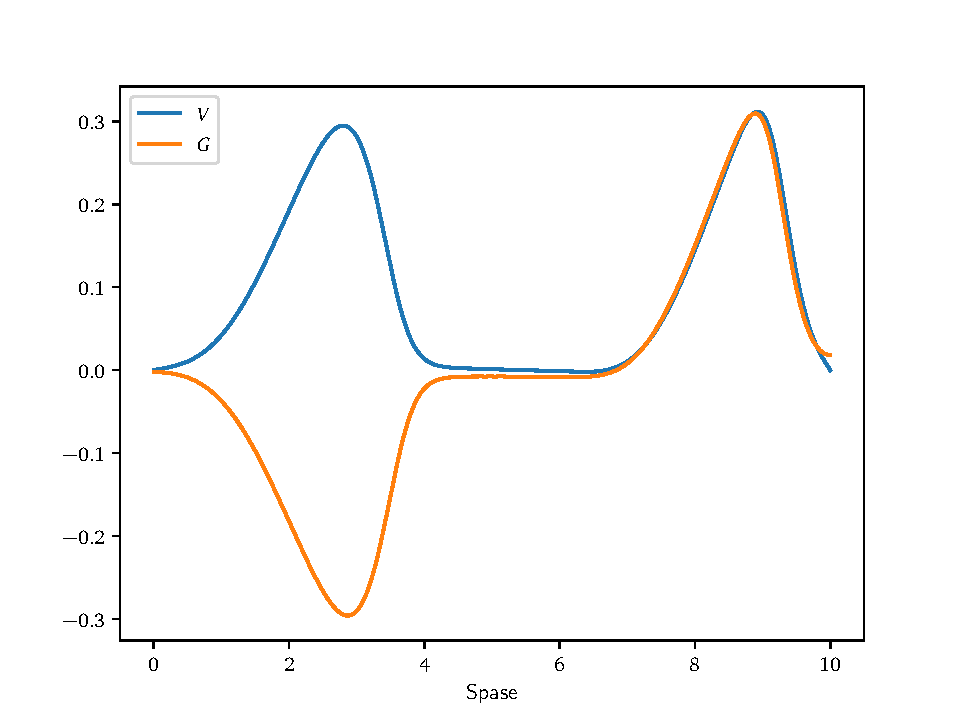
\includegraphics[scale=0.9]{pics_1d_cut/cut_4_1_1_0.1_3.pdf}}
\caption{Срез для $t=3$.}
\end{figure}

\begin{figure}[H]
\center{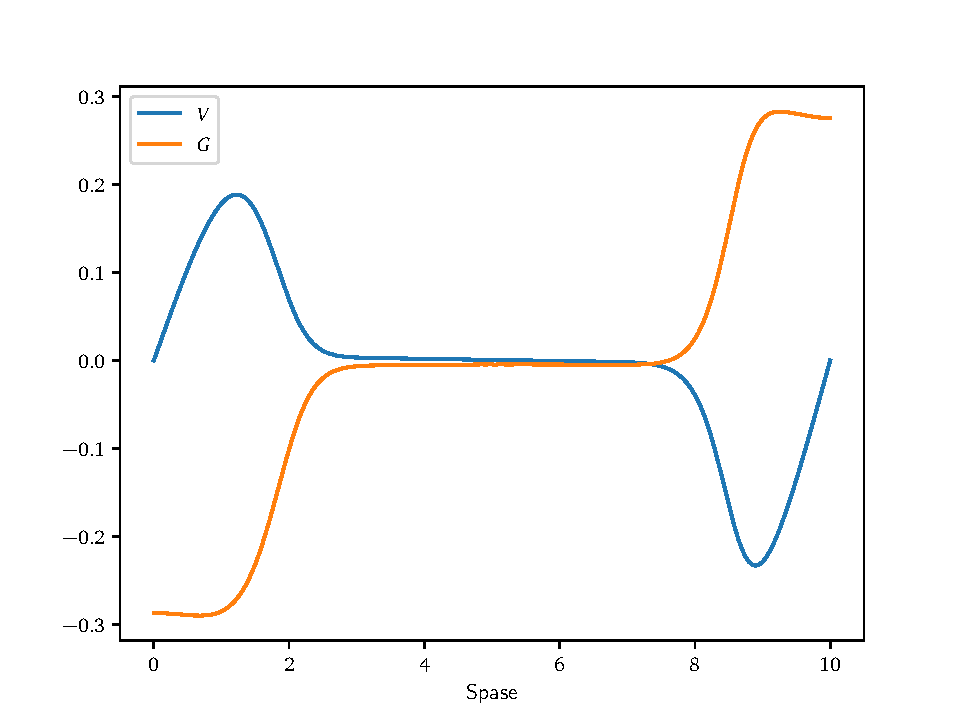
\includegraphics[scale=0.9]{pics_1d_cut/cut_4_1_1_0.1_4.pdf}}
\caption{Срез для $t=5$.}
\end{figure}

\begin{figure}[H]
\center{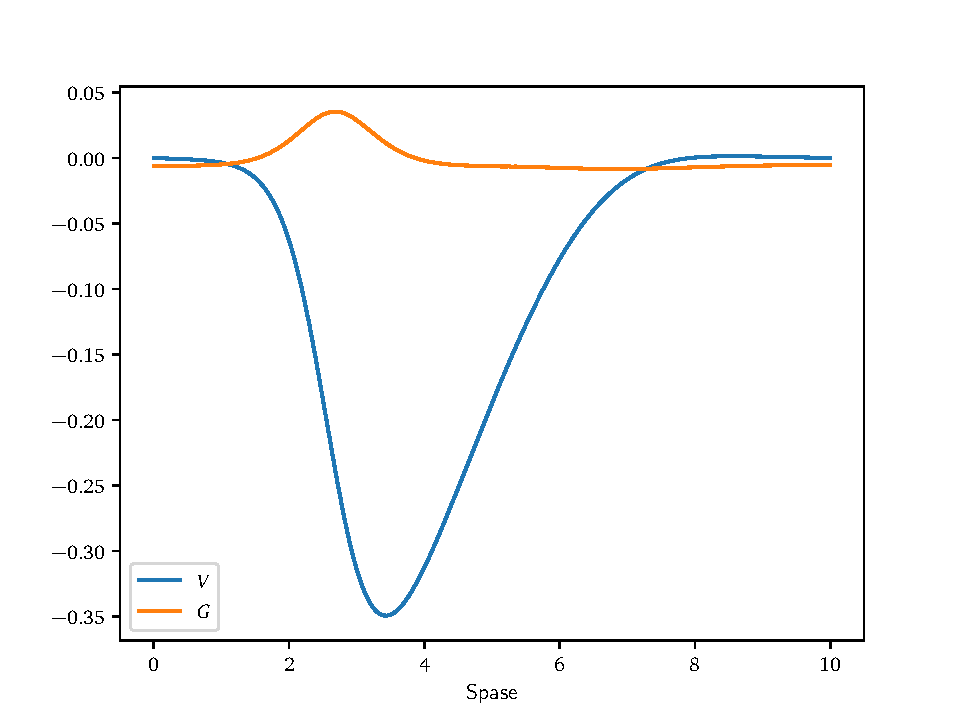
\includegraphics[scale=0.9]{pics_1d_cut/cut_4_1_1_0.1_5.pdf}}
\caption{Срез для $t=10$.}
\end{figure}

\begin{figure}[H]
\center{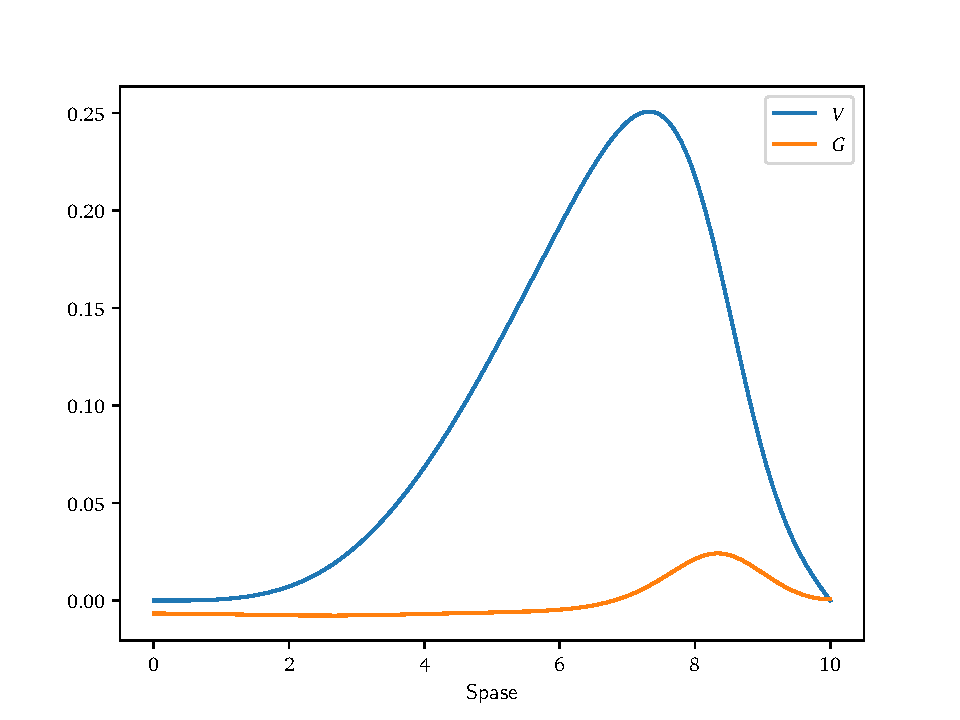
\includegraphics[scale=0.9]{pics_1d_cut/cut_4_1_1_0.1_6.pdf}}
\caption{Срез для $t=20$.}
\end{figure}

\begin{figure}[H]
\center{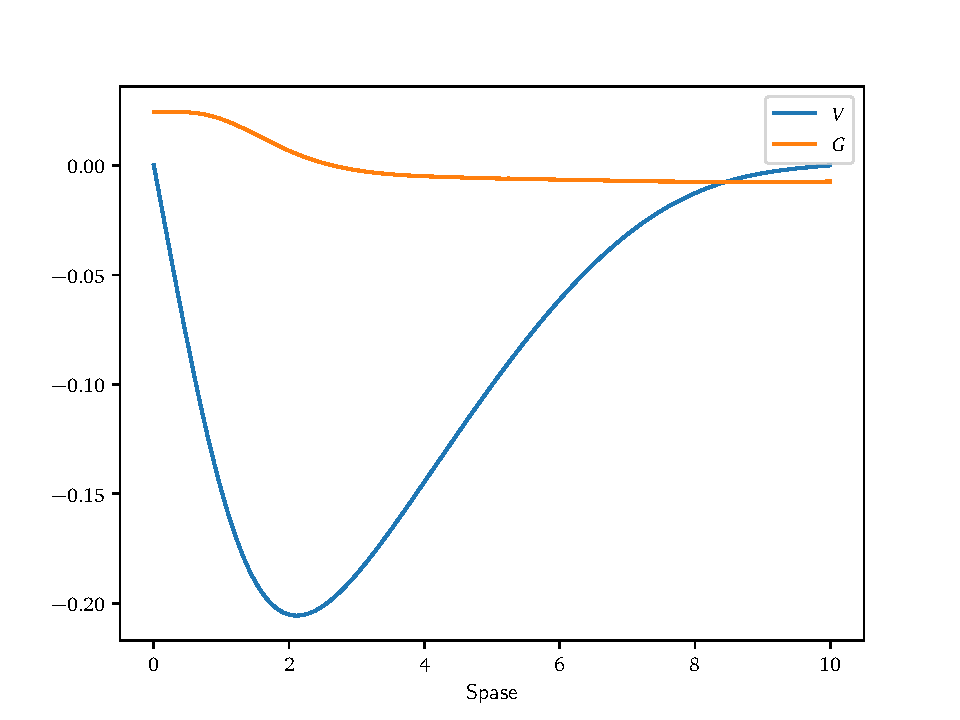
\includegraphics[scale=0.9]{pics_1d_cut/cut_4_1_1_0.1_7.pdf}}
\caption{Срез для $t=30$.}
\end{figure}

\begin{figure}[H]
\center{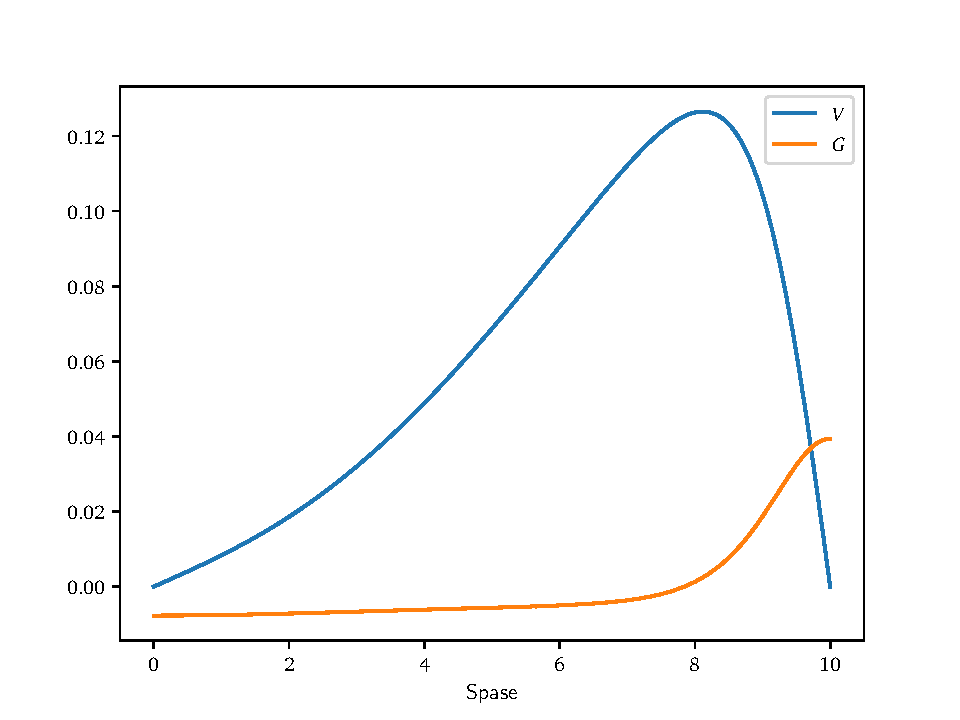
\includegraphics[scale=0.9]{pics_1d_cut/cut_4_1_1_0.1_8.pdf}}
\caption{Срез для $t=60$.}
\end{figure}

\begin{figure}[H]
\center{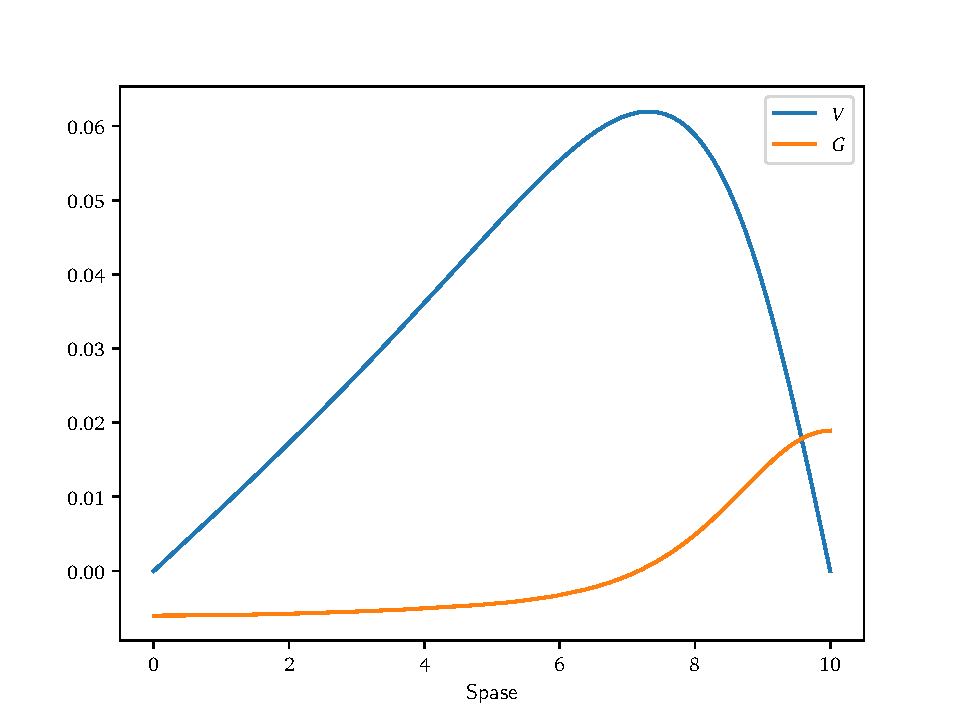
\includegraphics[scale=0.9]{pics_1d_cut/cut_4_1_1_0.1_9.pdf}}
\caption{Срез для $t=120$.}
\end{figure}

\begin{figure}[H]
\center{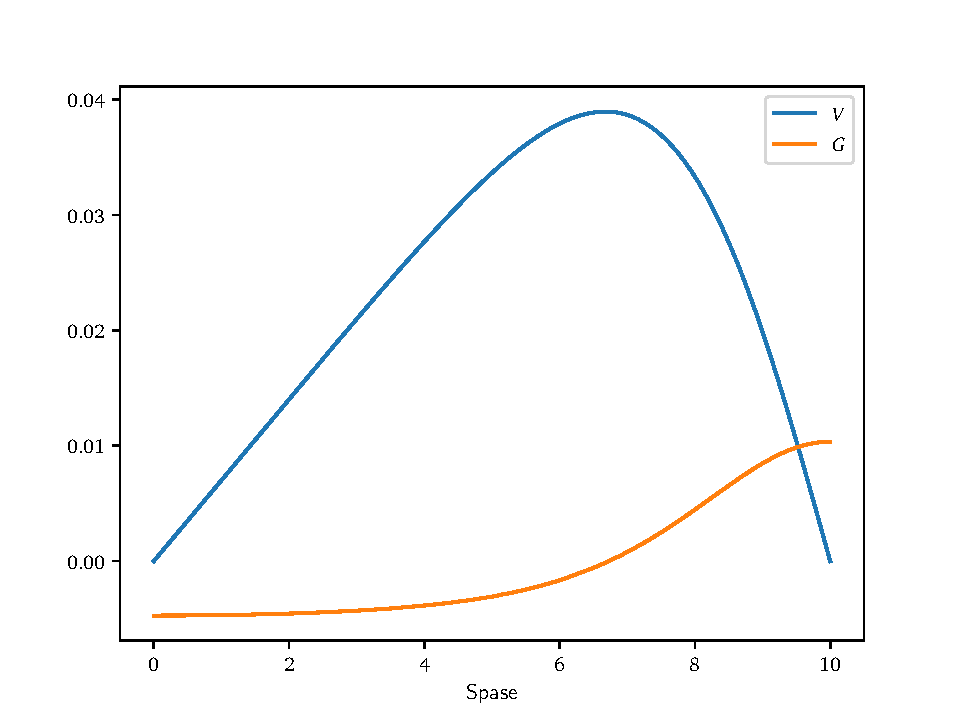
\includegraphics[scale=0.9]{pics_1d_cut/cut_4_1_1_0.1_10.pdf}}
\caption{Срез для $t=180$.}
\end{figure}

\begin{figure}[H]
\center{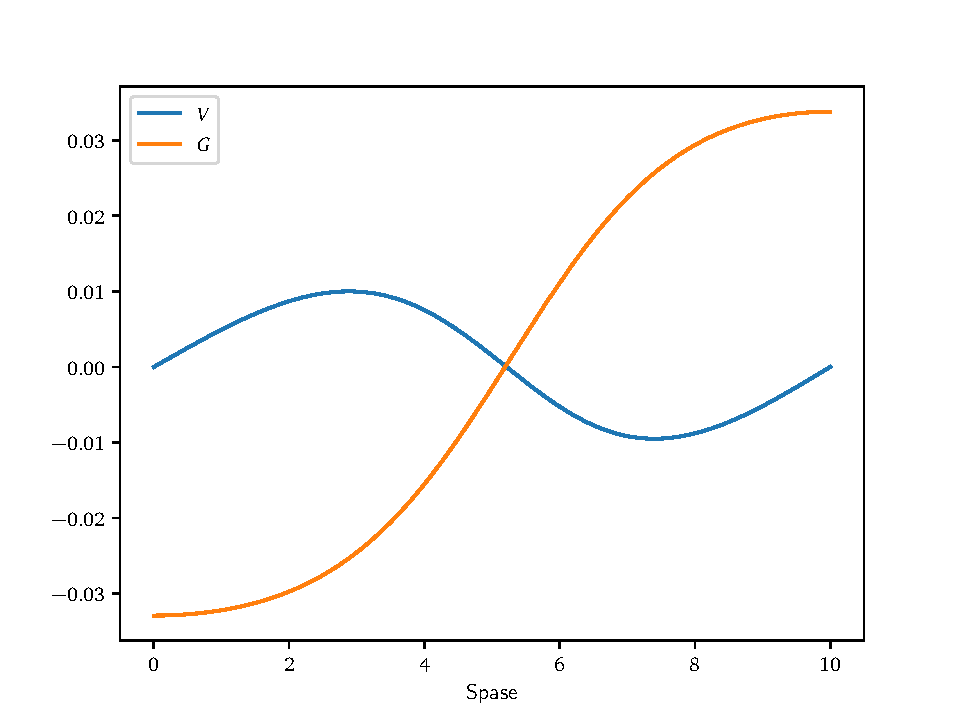
\includegraphics[scale=0.9]{pics_1d_cut/cut_4_1_1_0.1_11.pdf}}
\caption{Срез для $t=184.35$.}
\end{figure}


\subsubsection{Цикличность решения}
Для изучения зависимости периода от параметров $\mu$ и $C$ 
рассмотрим графики $V$ и $G$ для $T = 60$.
\begin{figure}[H]
\center{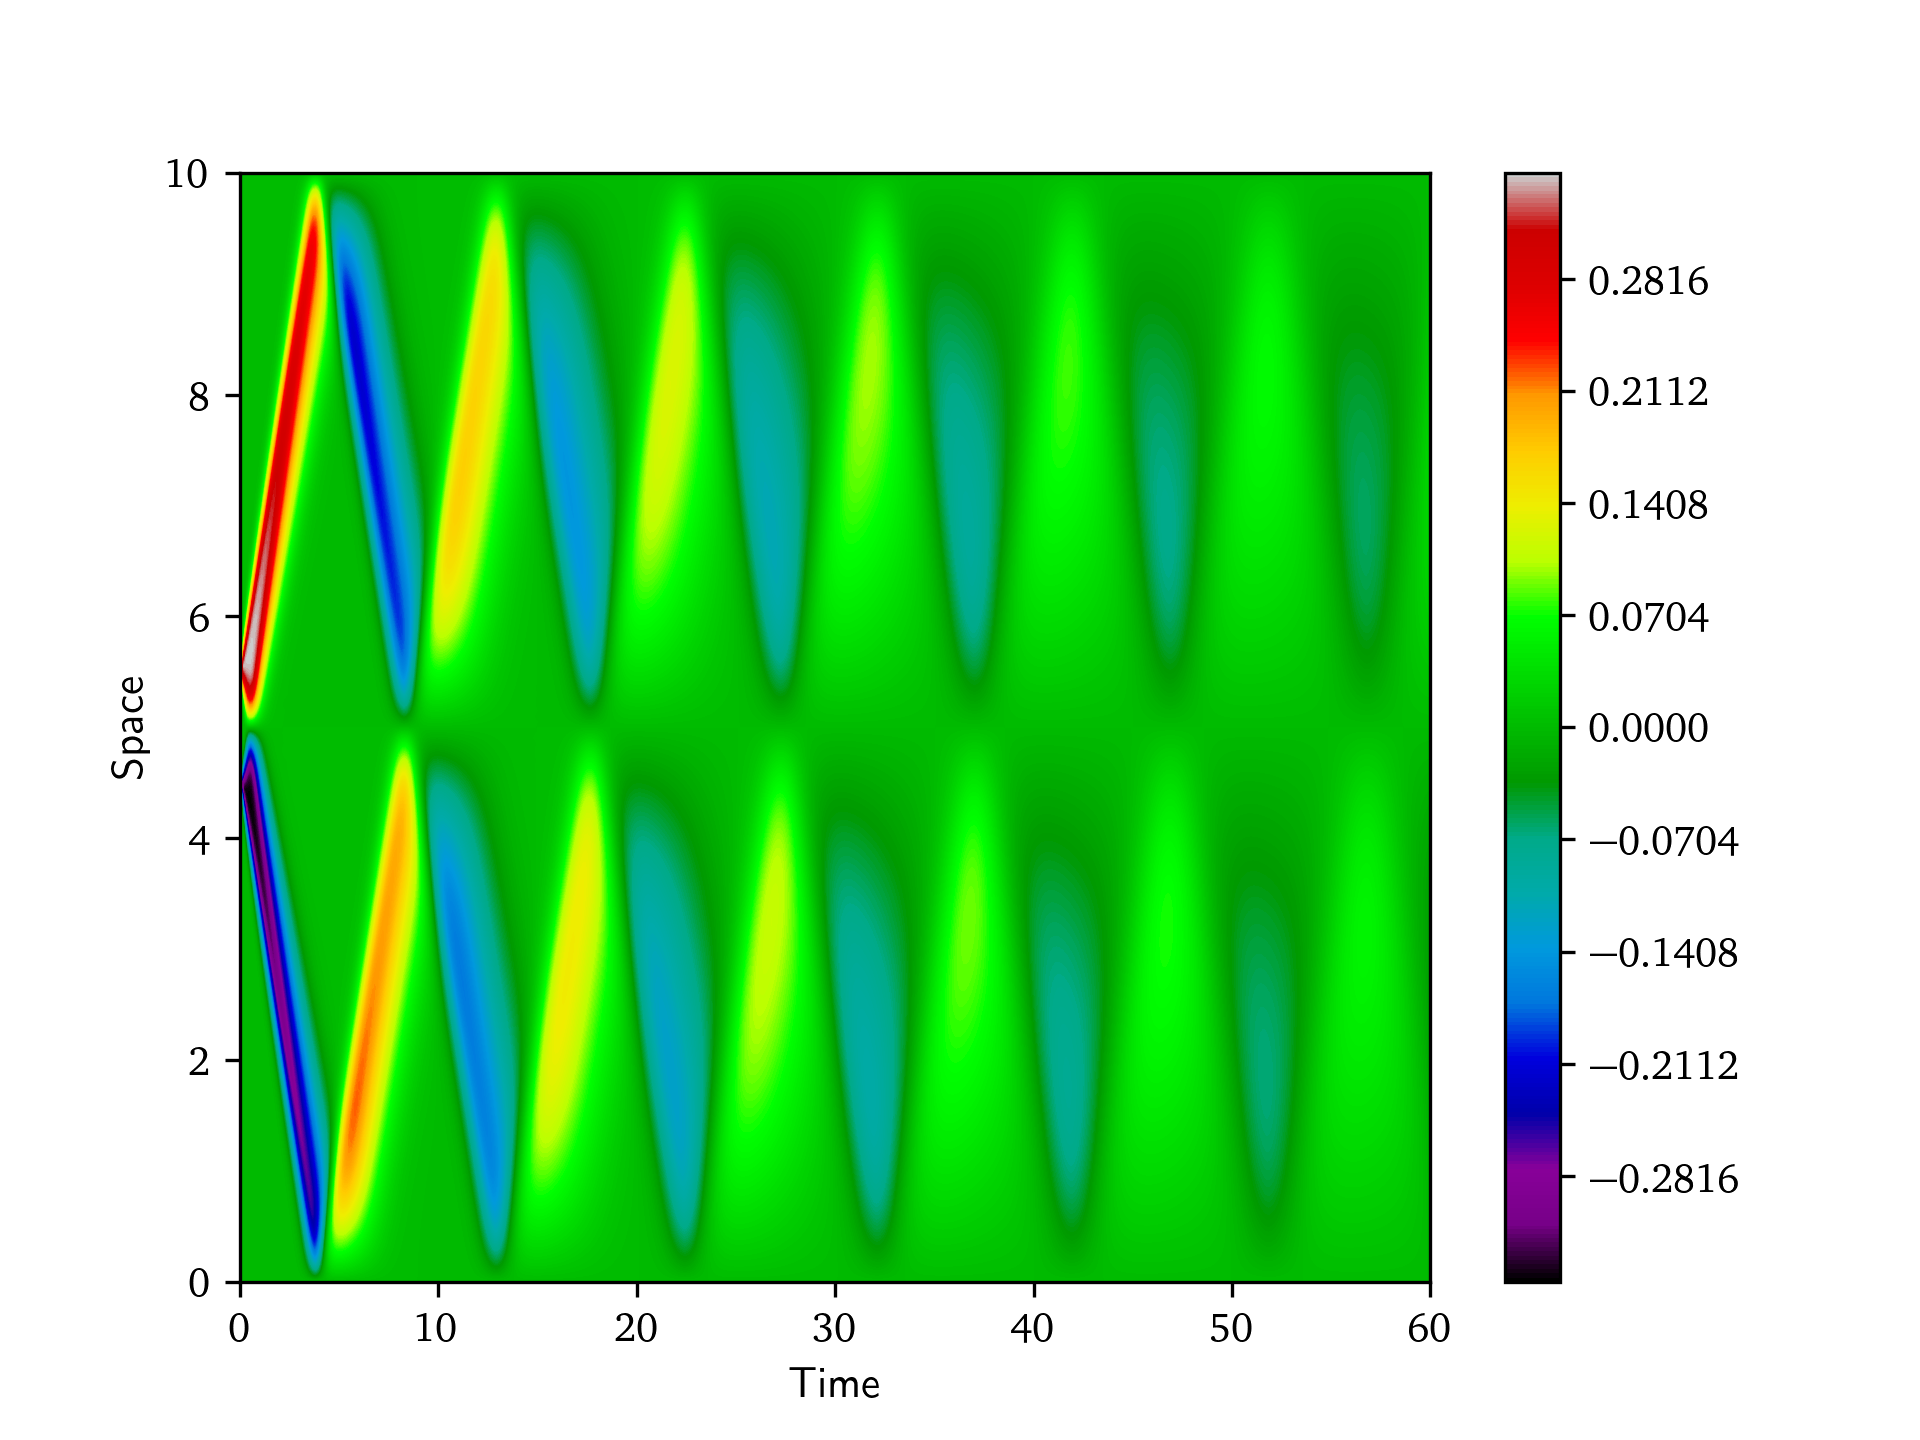
\includegraphics[scale=0.85]{pics_2d/plot_V_3_1_1_0.1.png}}
\caption{График $V$ для $T = 60$ при $C = 1$, $\gamma = 1$ и~$\mu = 0.1$.}
\end{figure}
\begin{figure}[H]
\center{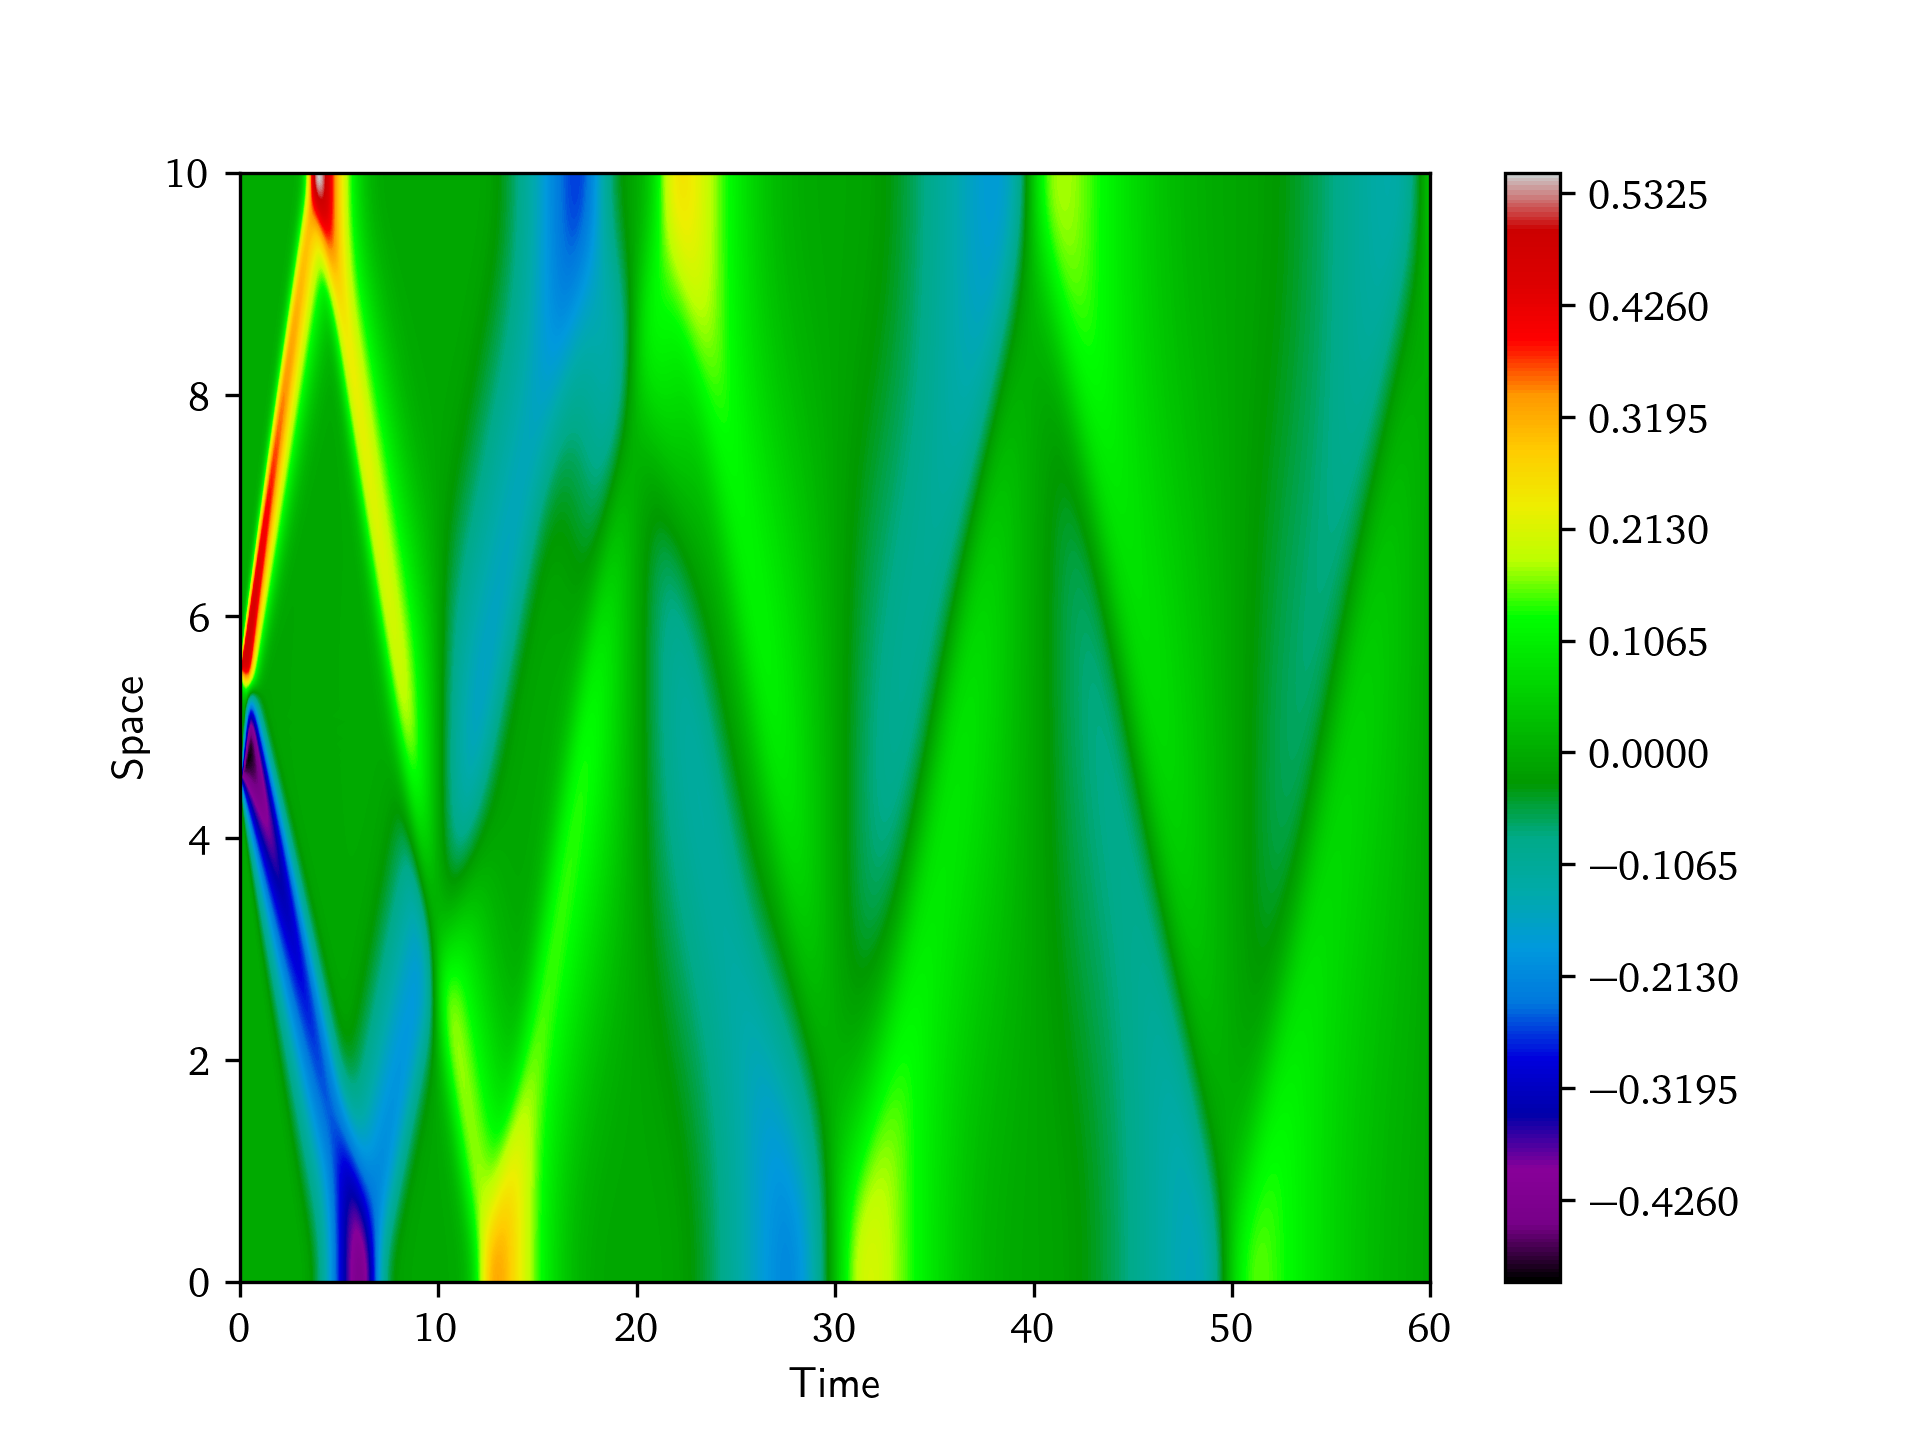
\includegraphics[scale=0.85]{pics_2d/plot_G_4_1_1_0.1.png}}
\caption{График $G$ для $T = 60$ при $C = 1$, $\gamma = 1$ и~$\mu = 0.1$.}
\end{figure}

\begin{figure}[H]
\center{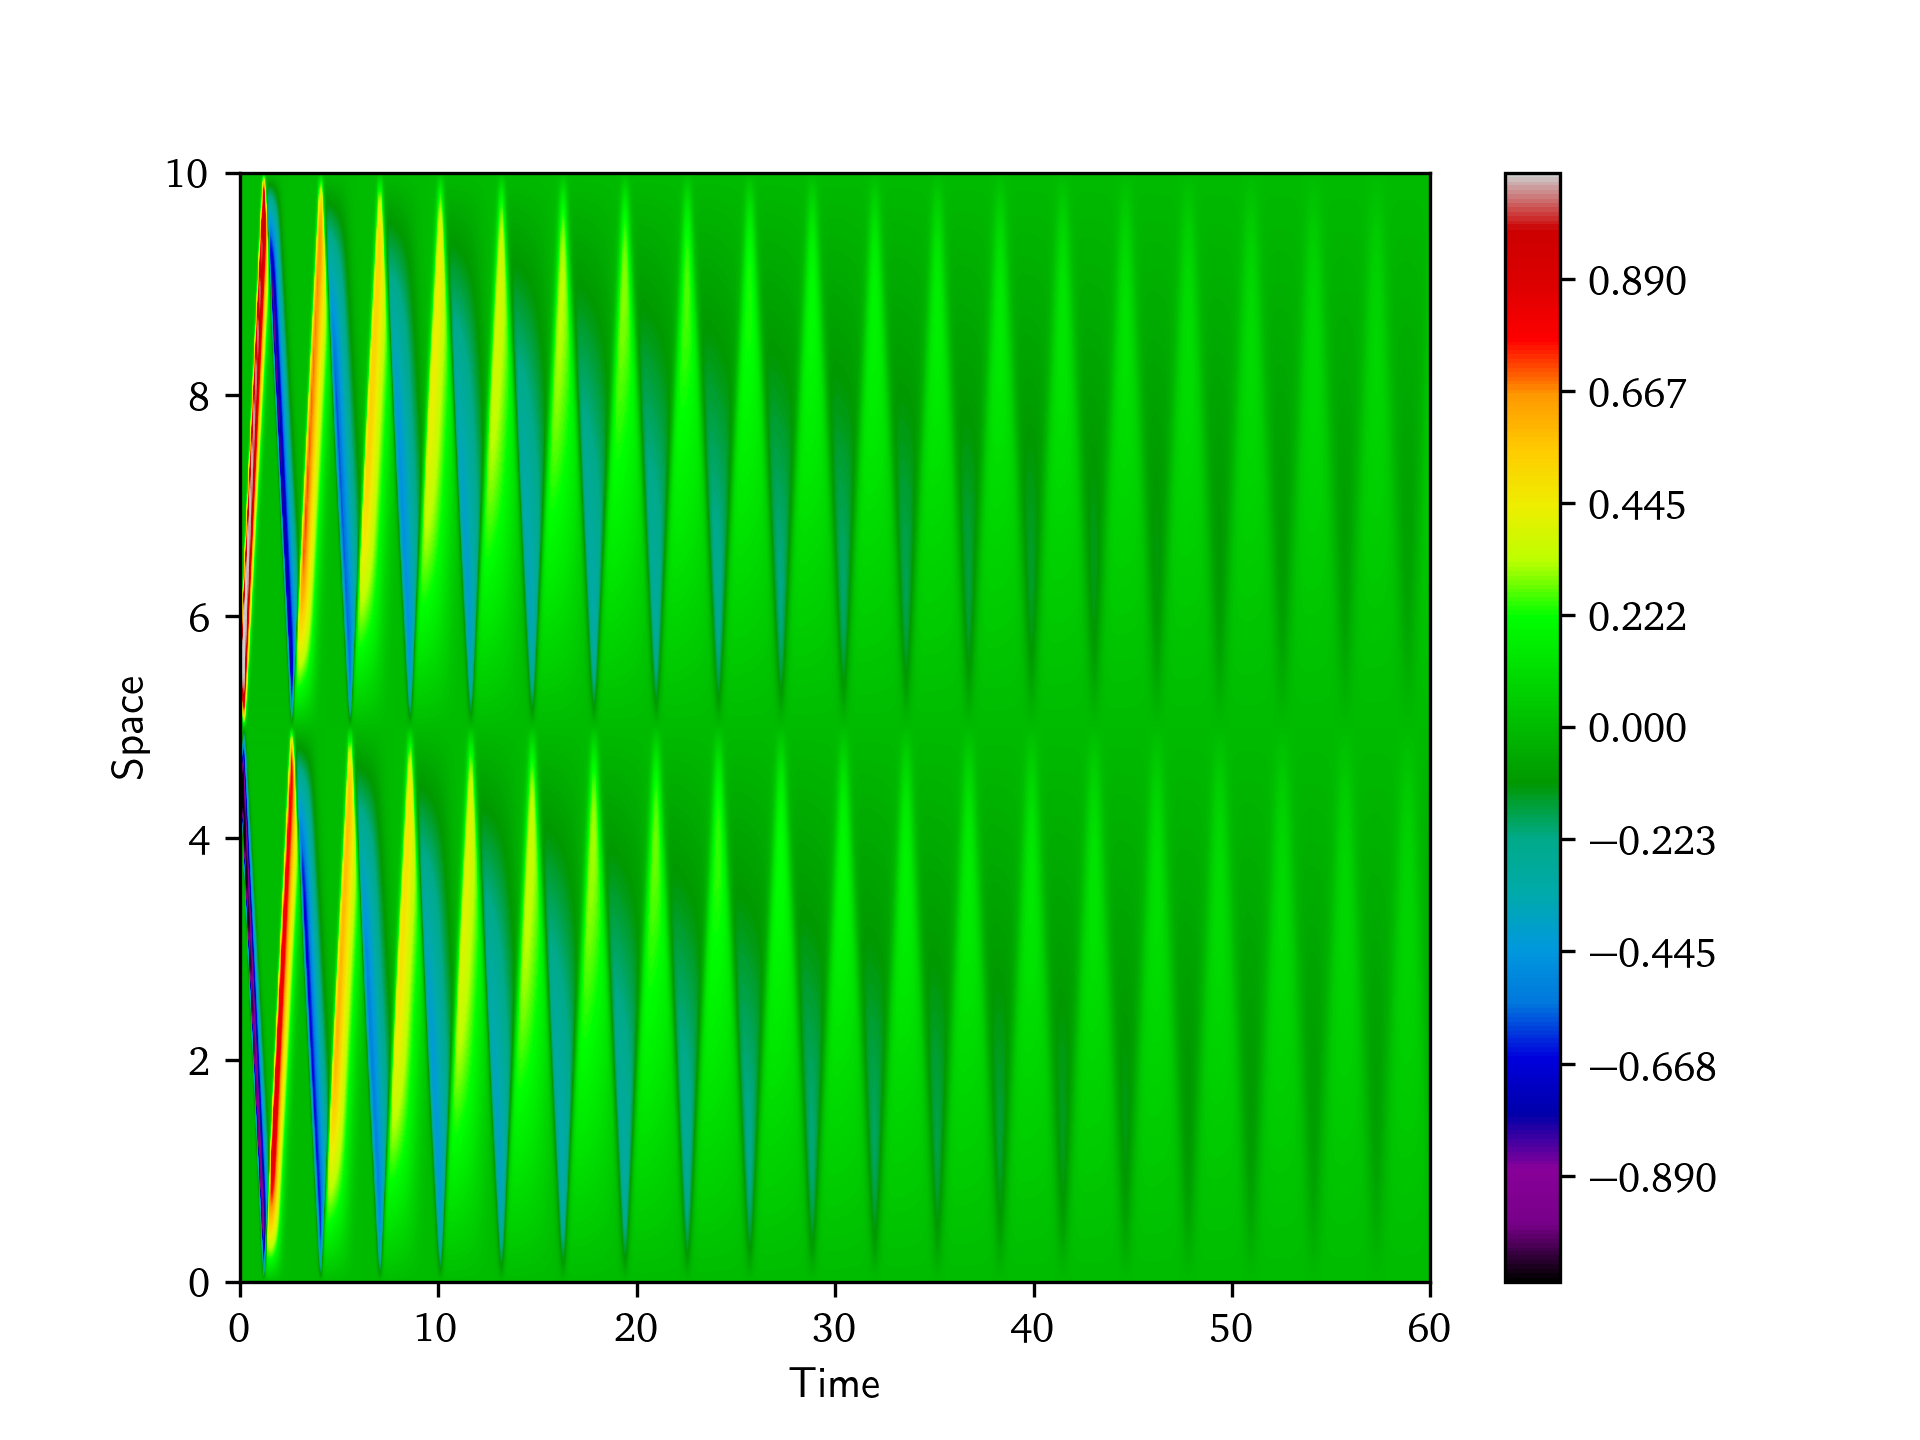
\includegraphics[scale=0.85]{pics_2d/plot_V_3_10_1_0.1.png}}
\caption{График $V$ для $T = 60$ при $C = 10$, $\gamma = 1$ и~$\mu = 0.1$.}
\end{figure}
\begin{figure}[H]
\center{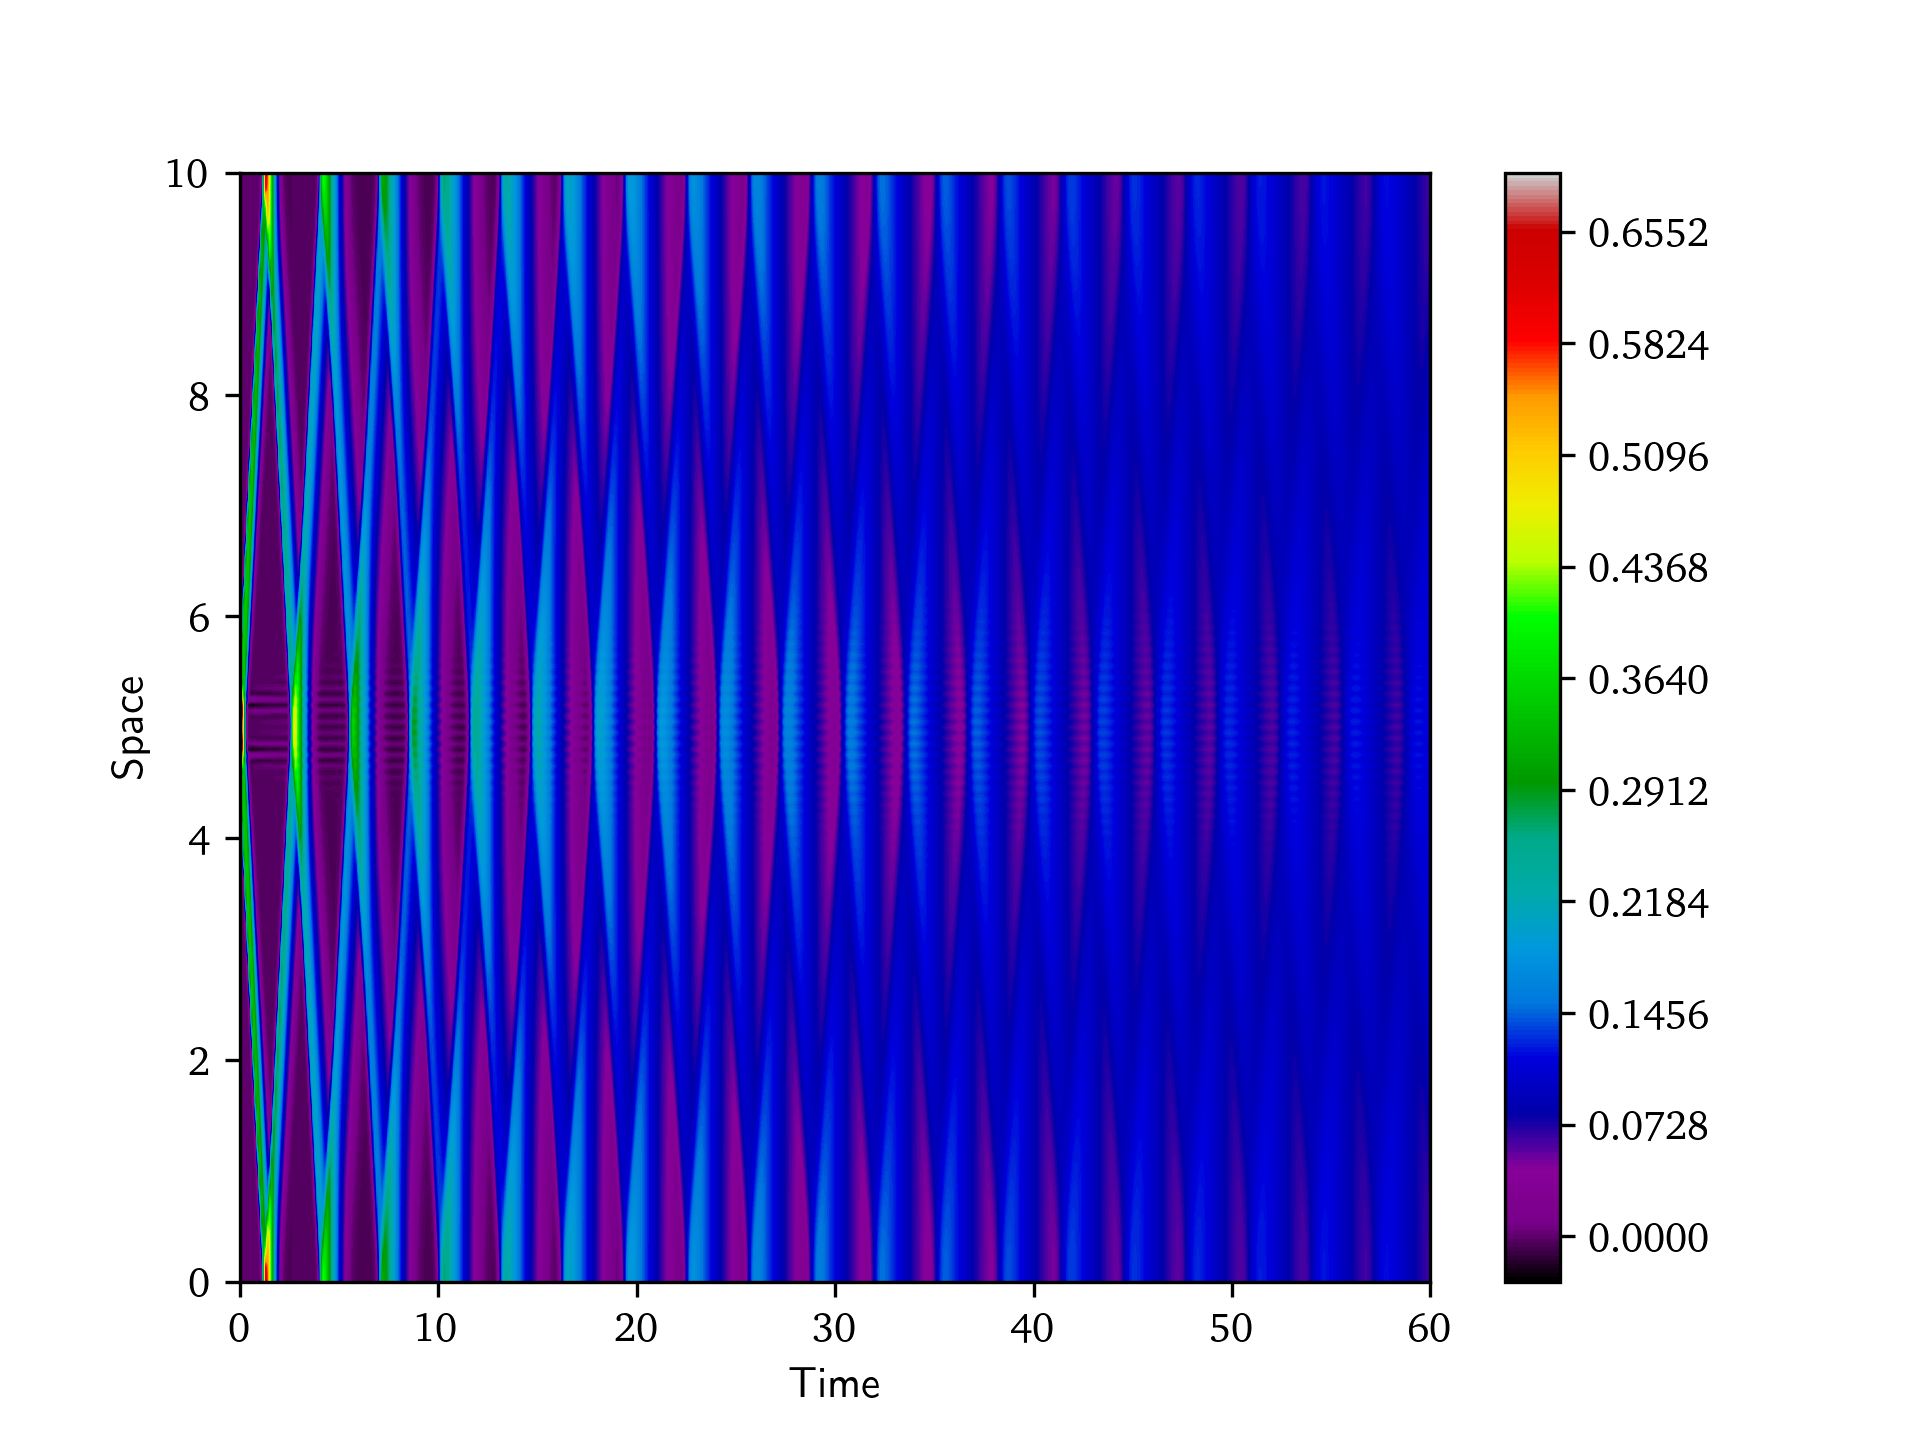
\includegraphics[scale=0.85]{pics_2d/plot_G_3_10_1_0.1.png}}
\caption{График $G$ для $T = 60$ при $C = 10$, $\gamma = 1$ и~$\mu = 0.1$.}
\end{figure}


\begin{figure}[H]
\center{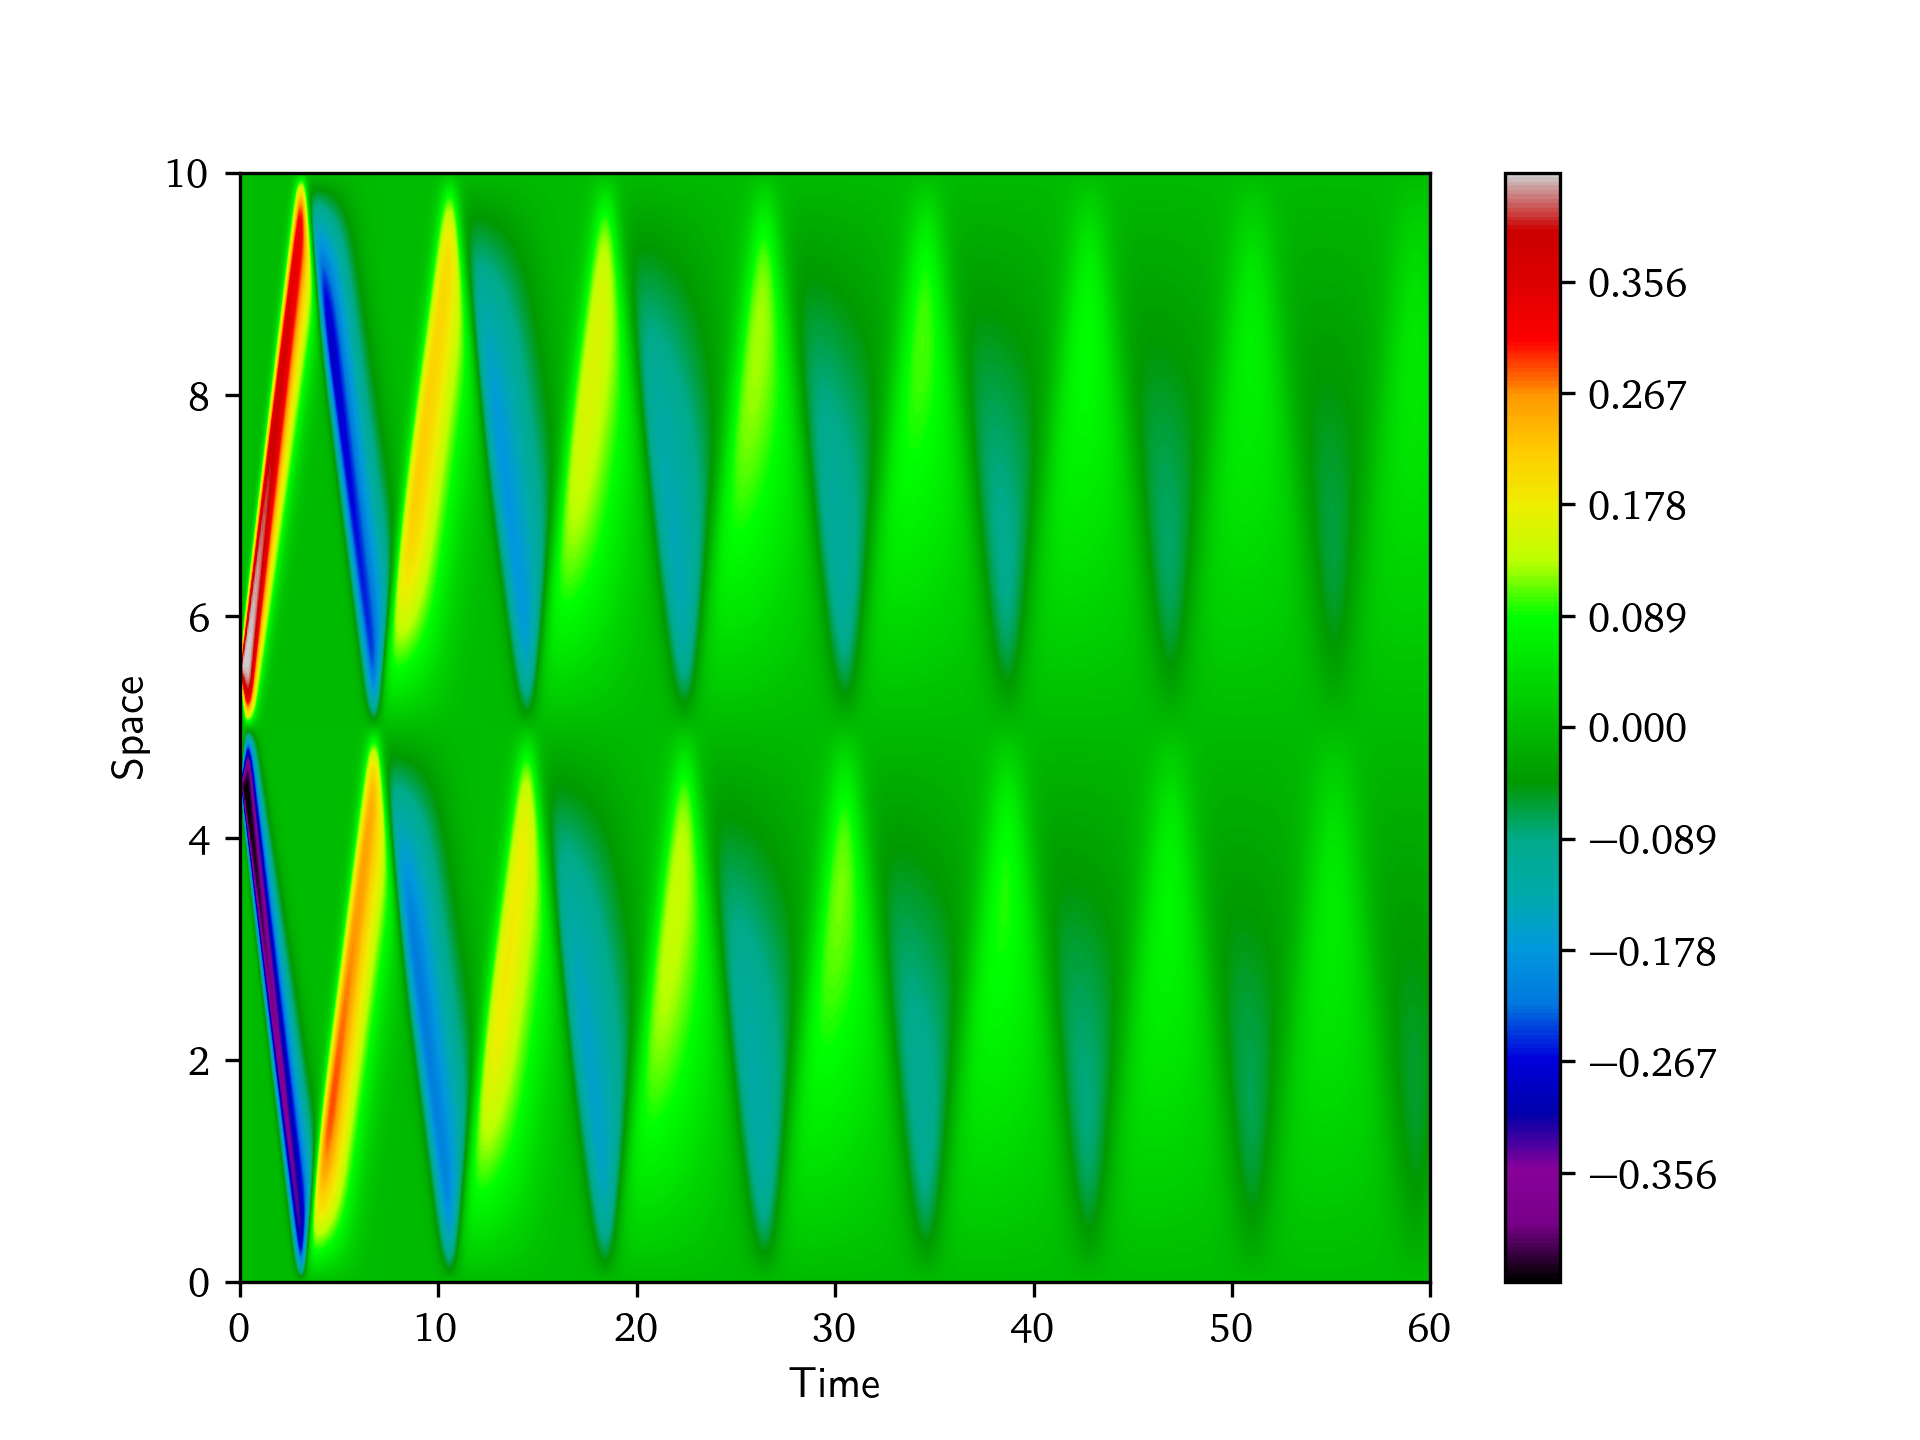
\includegraphics[scale=0.85]{pics_2d/plot_V_3_1_1.4_0.1.png}}
\caption{График $V$ для $T = 60$ при $C = 1$, $\gamma = 1.4$ и~$\mu = 0.1$.}
\end{figure}
\begin{figure}[H]
\center{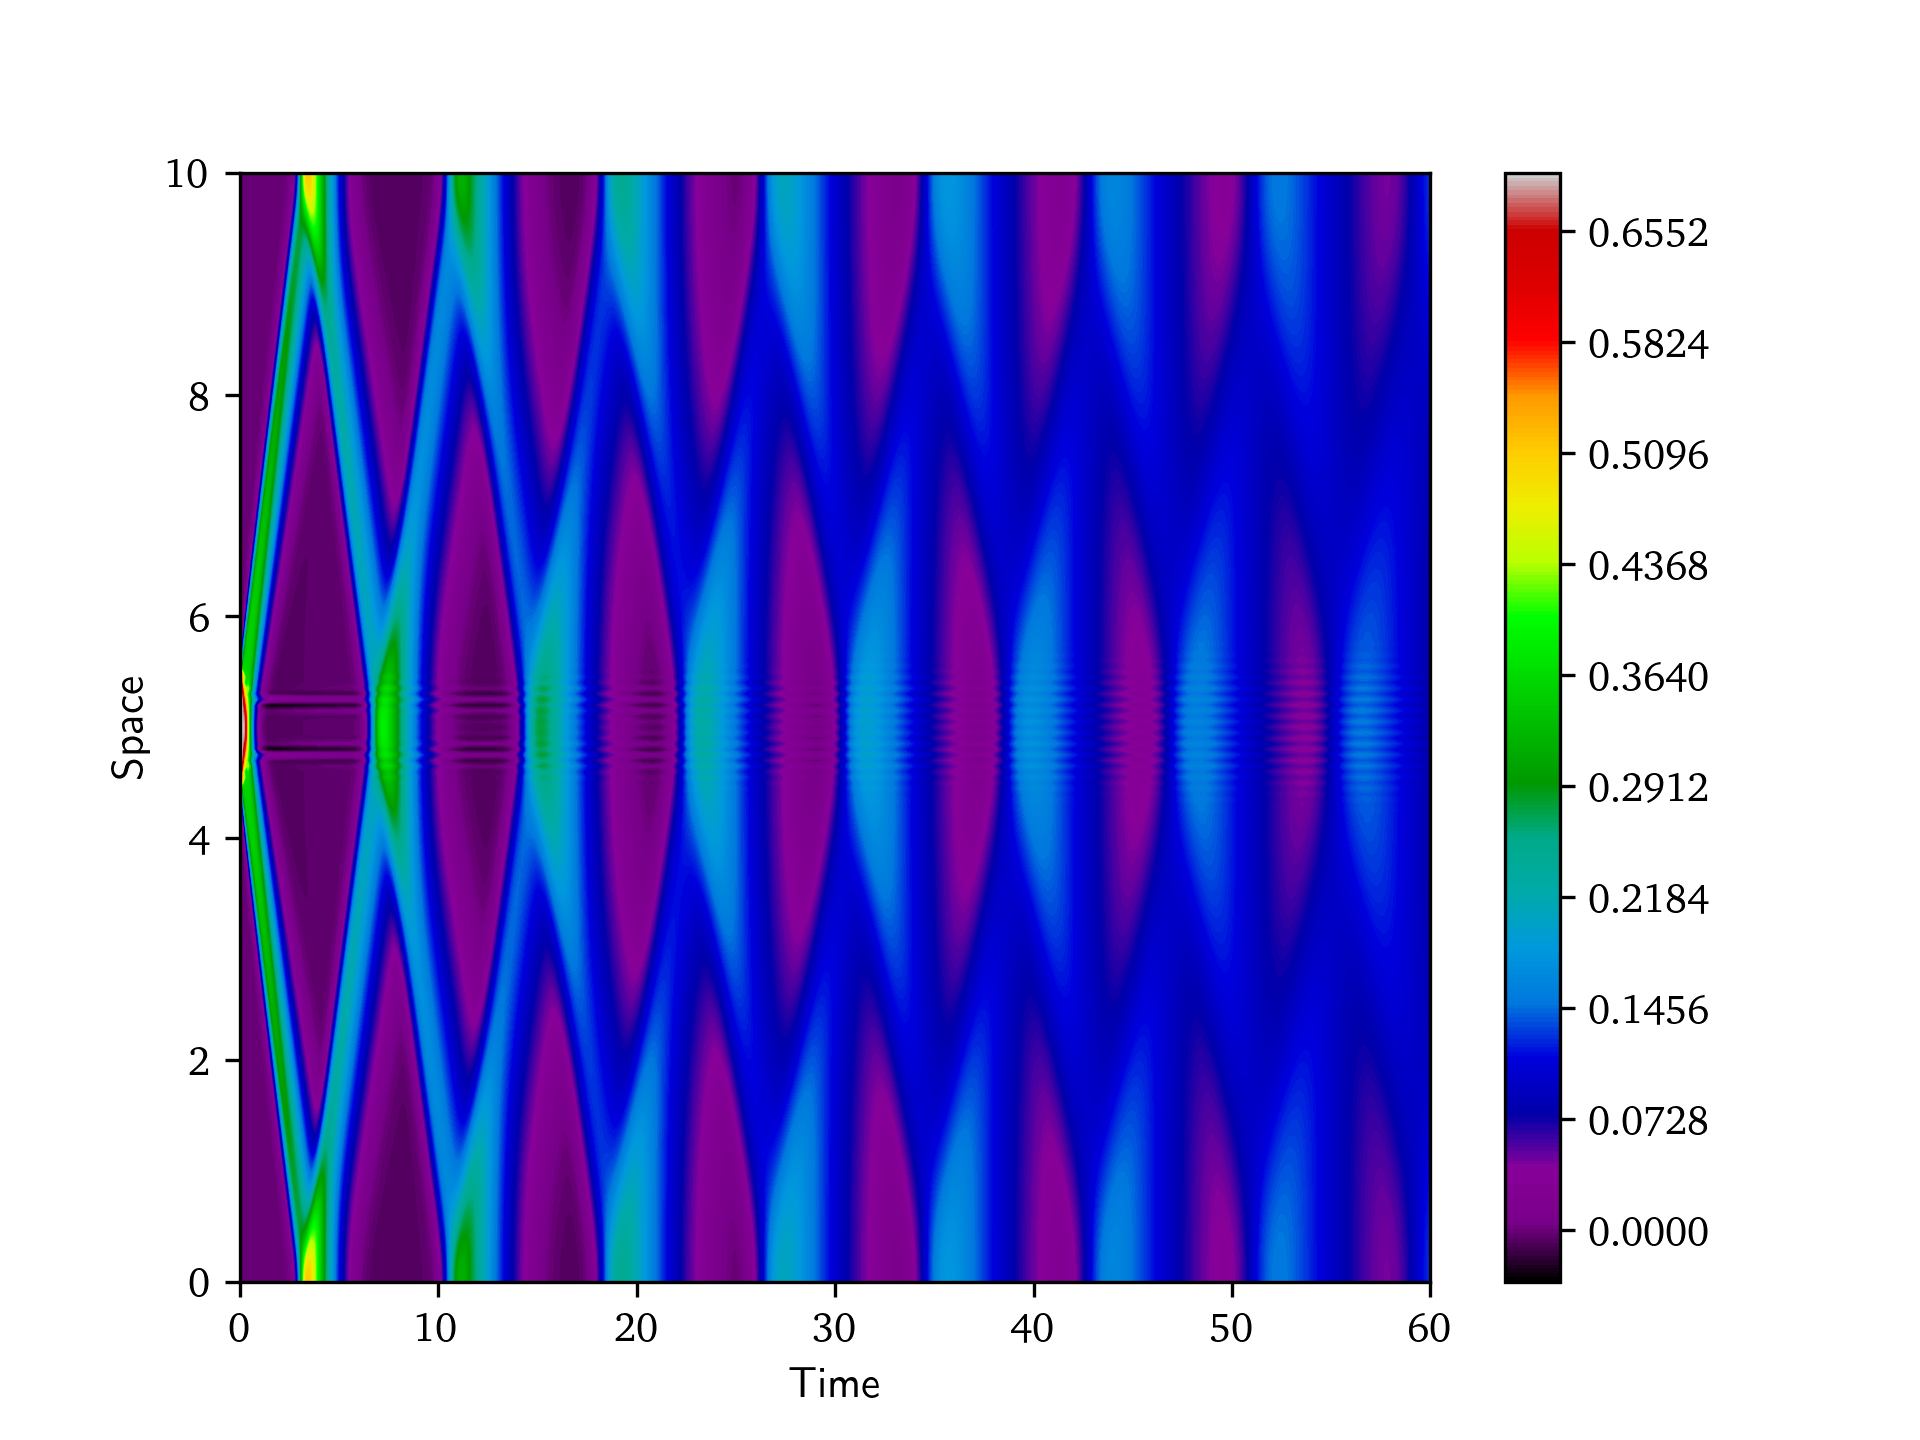
\includegraphics[scale=0.85]{pics_2d/plot_G_3_1_1.4_0.1.png}}
\caption{График $G$ для $T = 60$ при $C = 1$, $\gamma = 1.4$ и~$\mu = 0.1$.}
\end{figure}


\begin{figure}[H]
\center{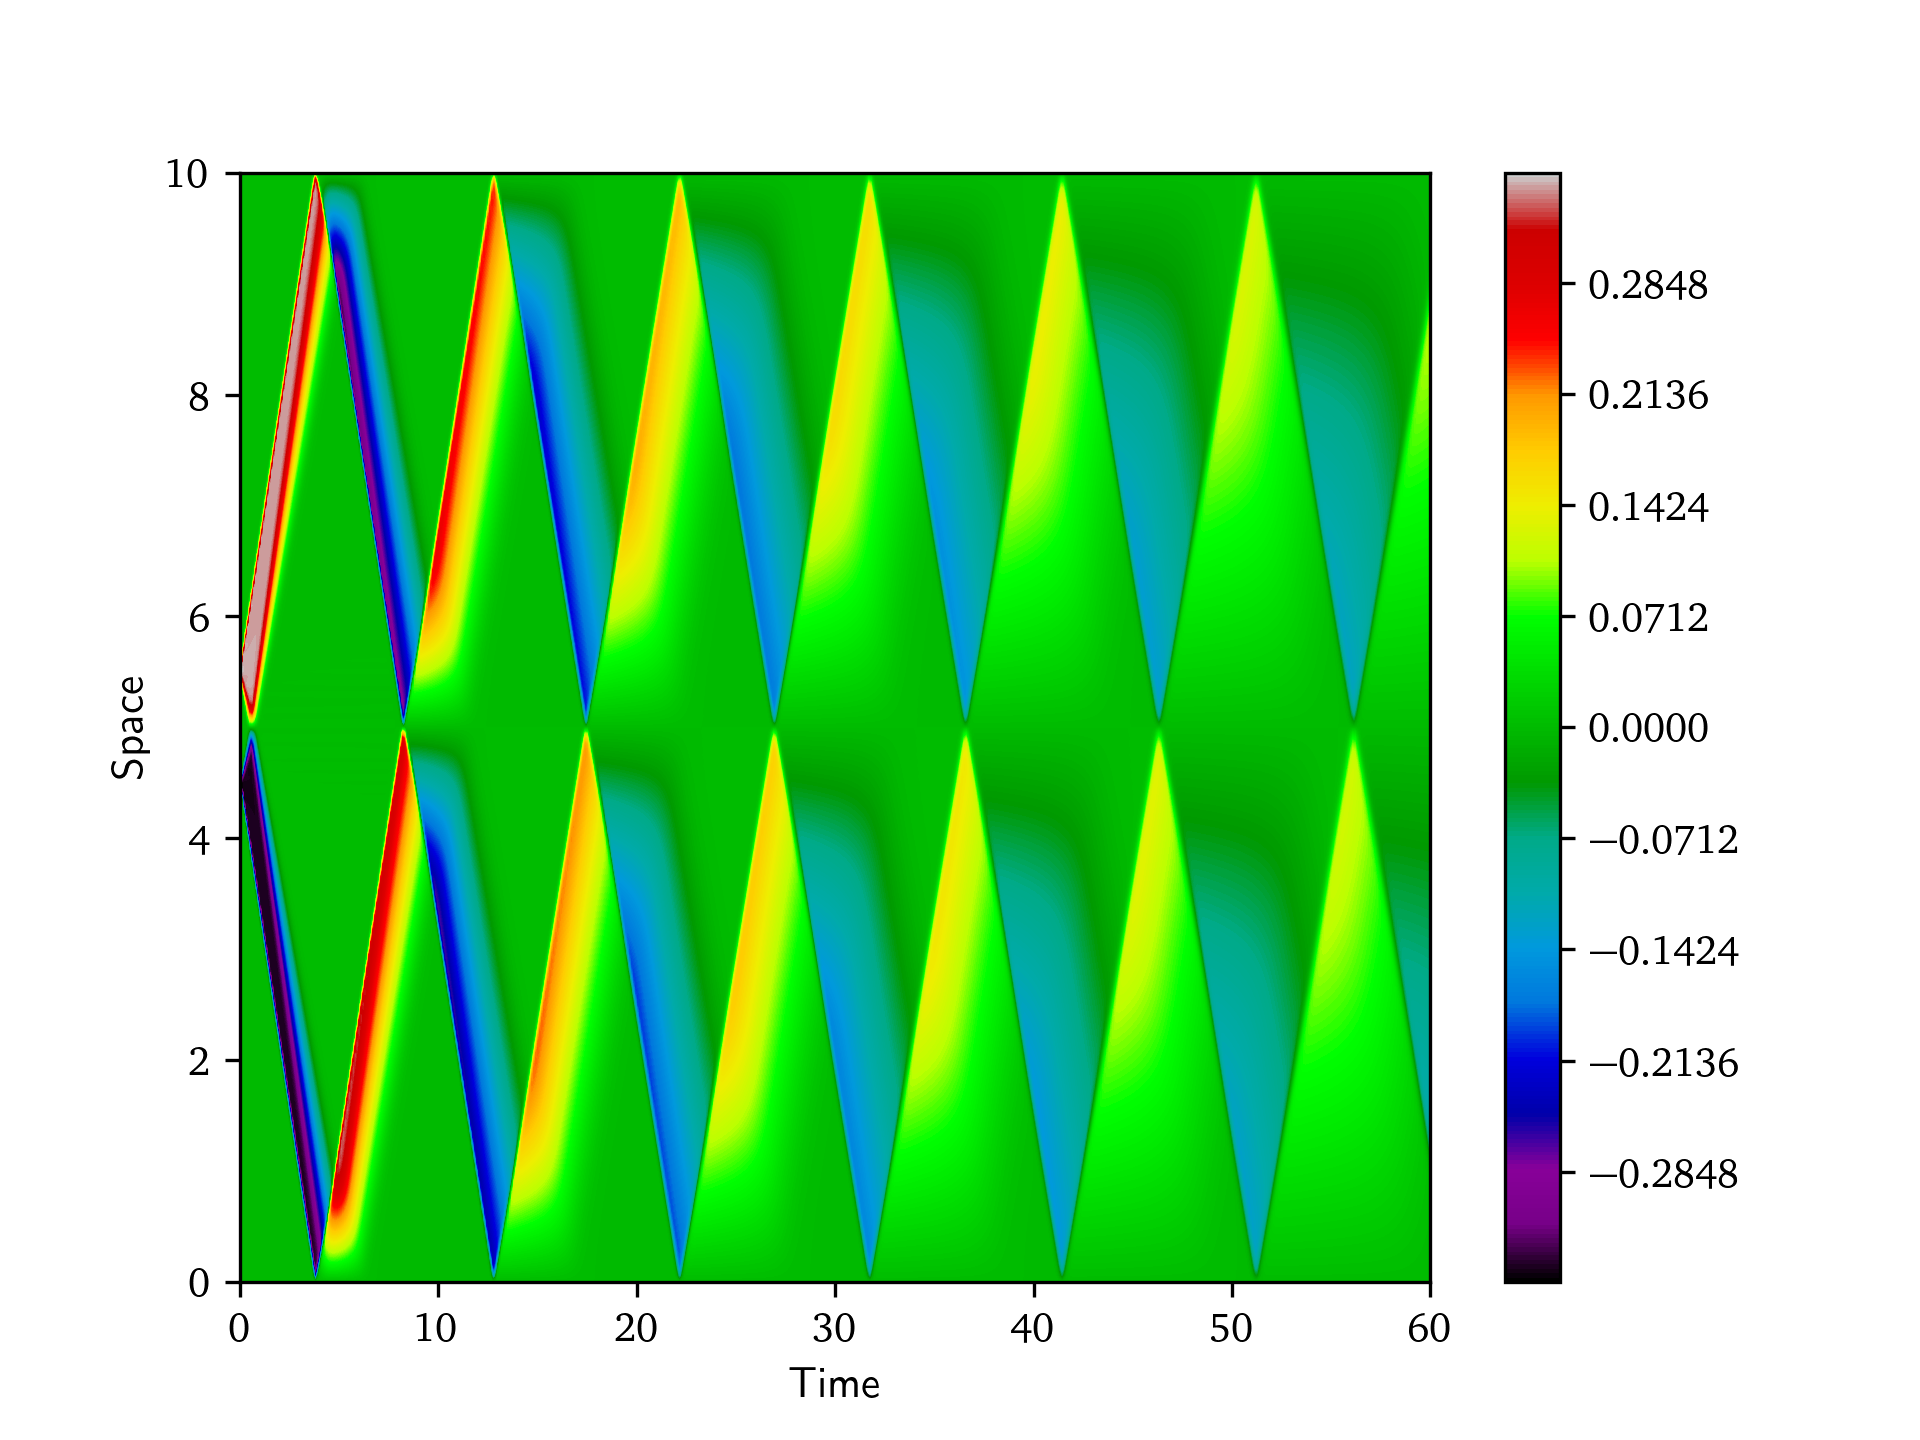
\includegraphics[scale=0.85]{pics_2d/plot_V_3_1_1_0.01.png}}
\caption{График $V$ для $T = 60$ при $C = 1$, $\gamma = 1$ и~$\mu = 0.01$.}
\end{figure}
\begin{figure}[H]
\center{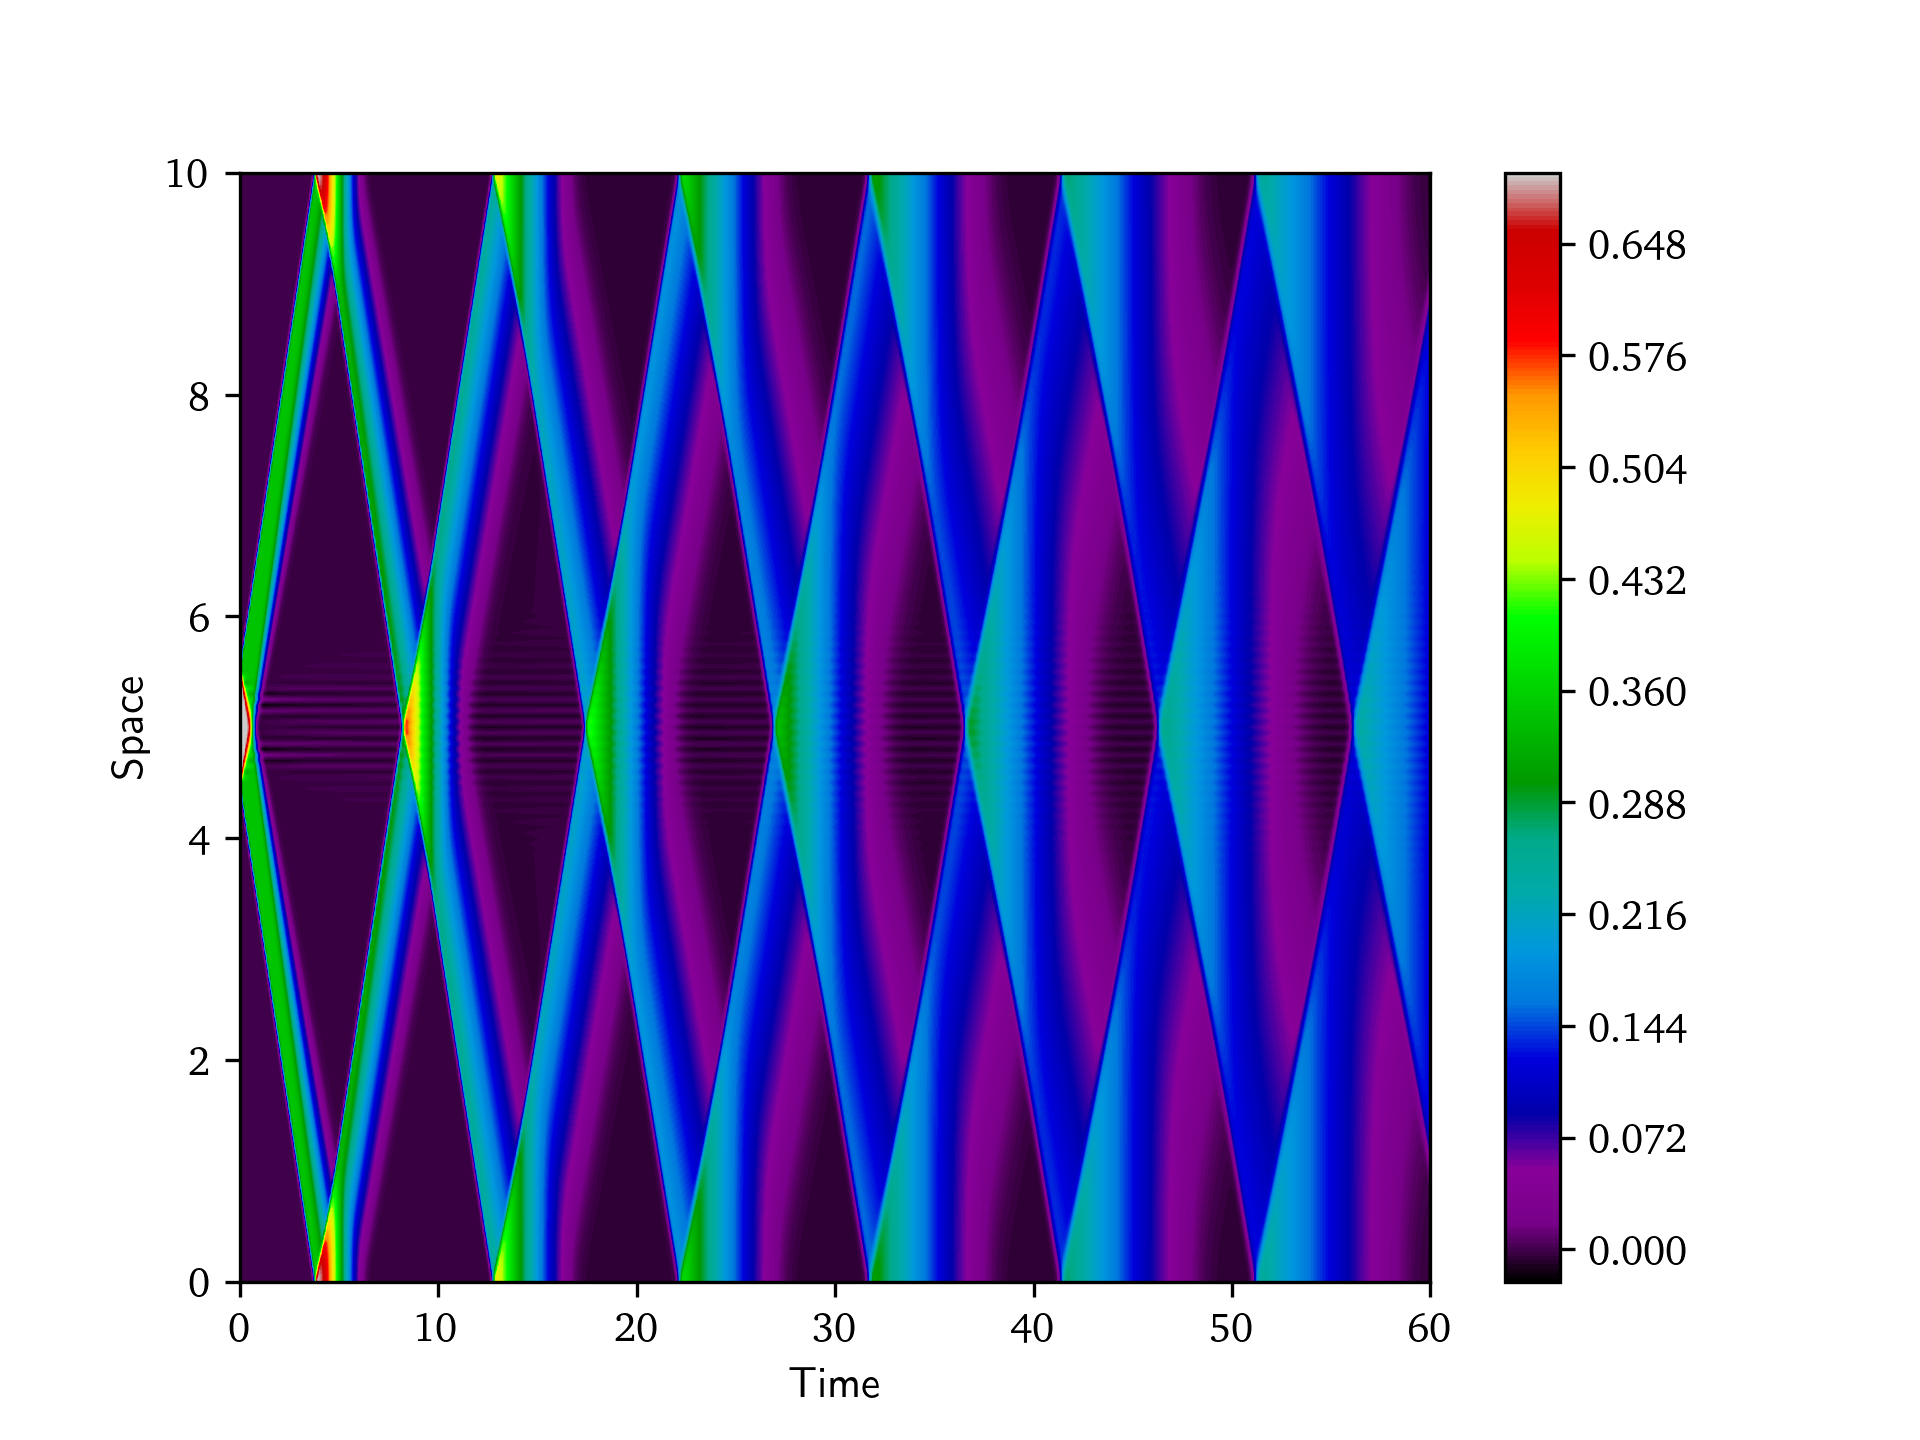
\includegraphics[scale=0.85]{pics_2d/plot_G_3_1_1_0.01.png}}
\caption{График $G$ для $T = 60$ при $C = 1$, $\gamma = 1$ и~$\mu = 0.01$.}
\end{figure}


\begin{figure}[H]
\center{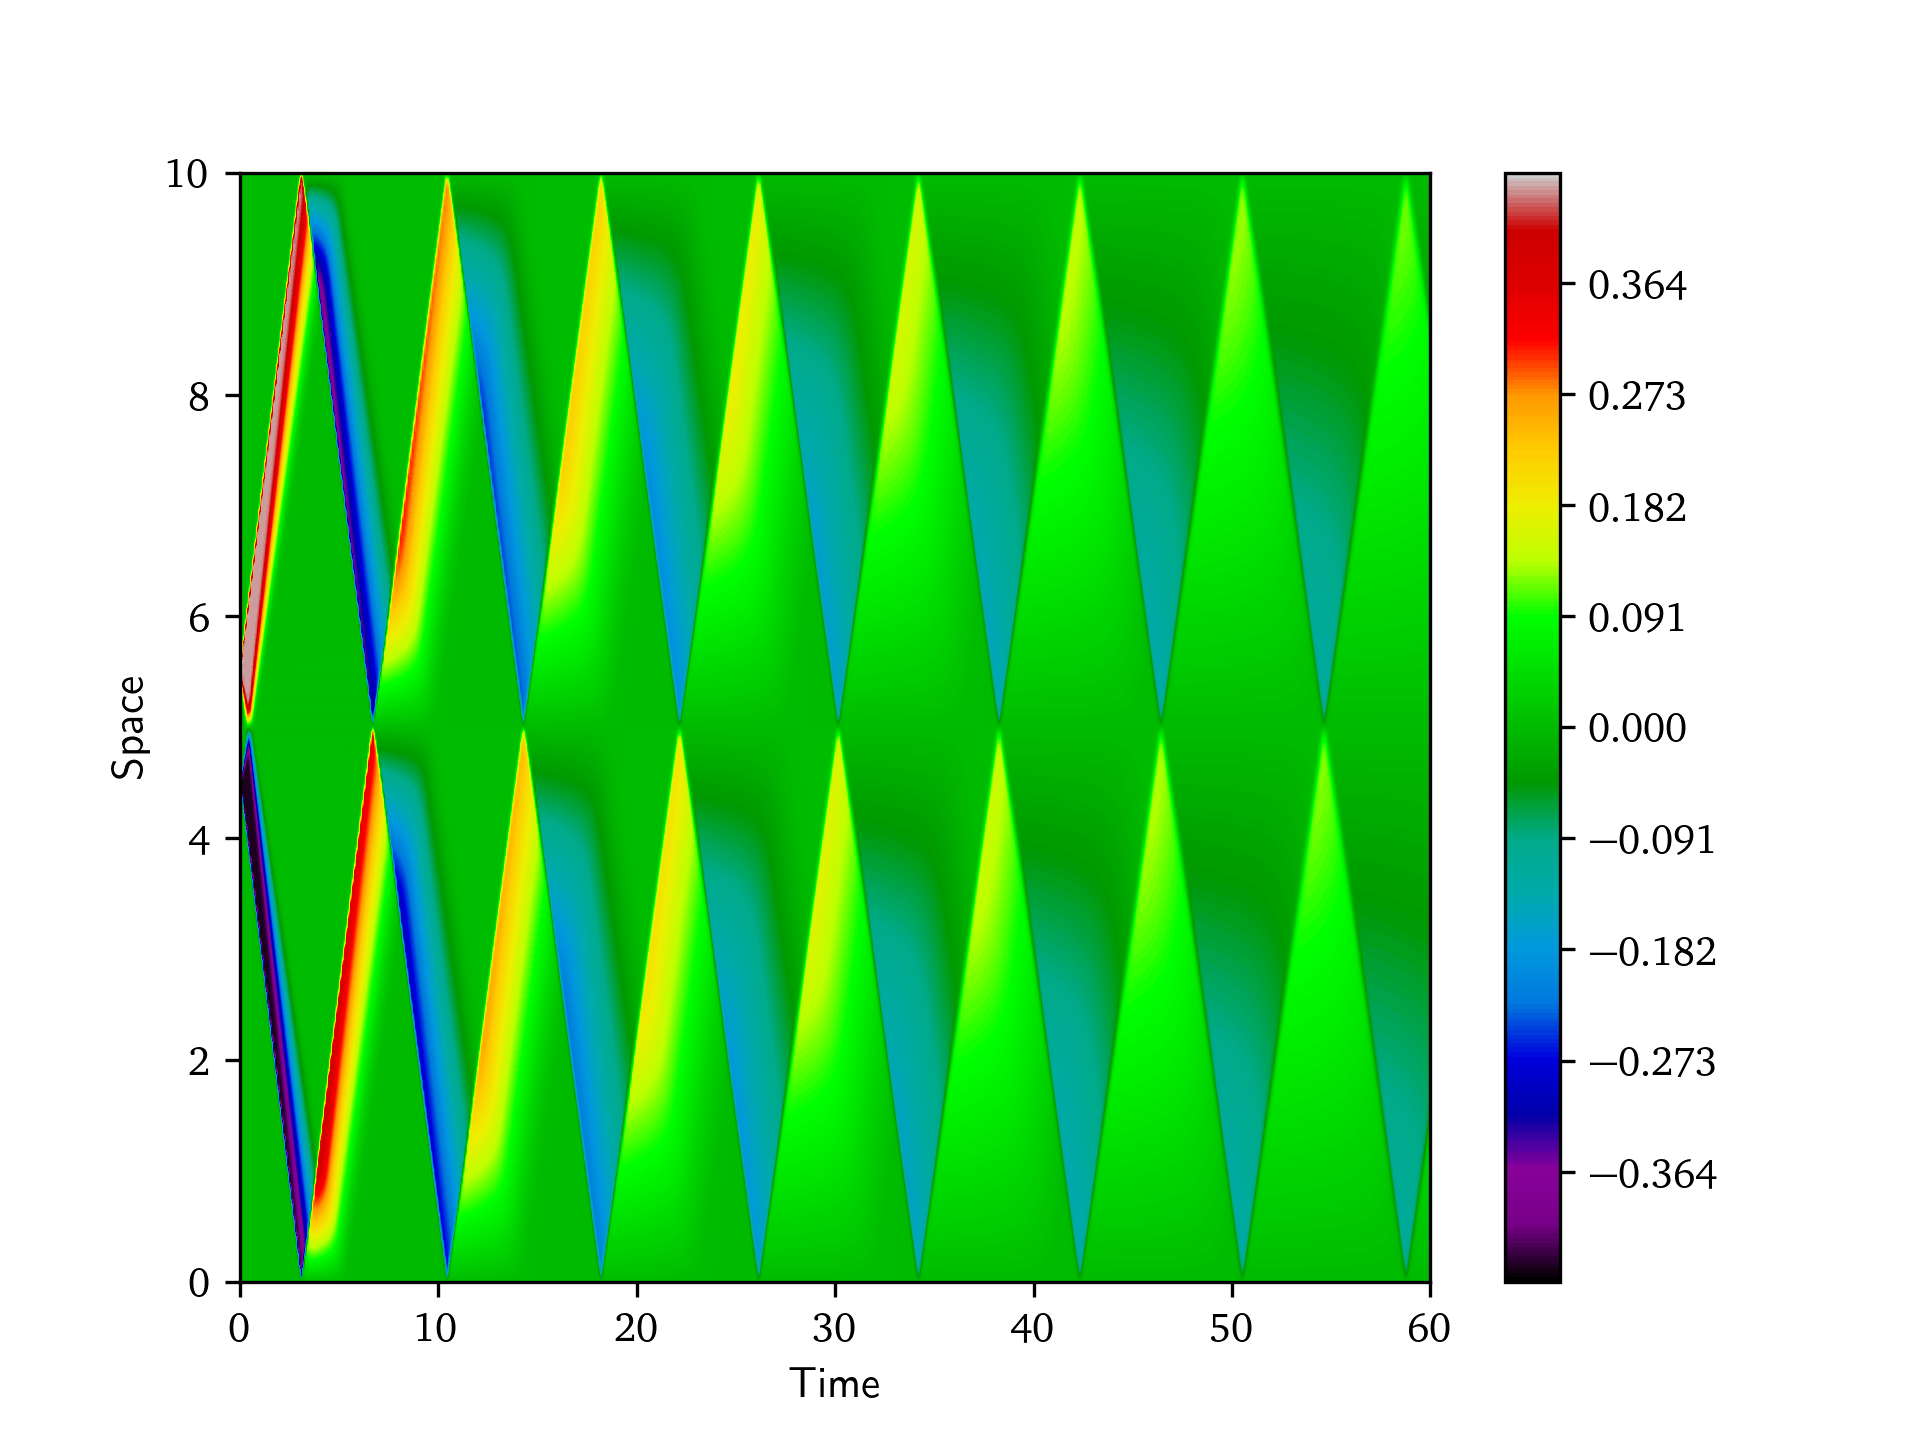
\includegraphics[scale=0.85]{pics_2d/plot_V_3_1_1.4_0.01.png}}
\caption{График $V$ для $T = 60$ при $C = 1$, $\gamma = 1.4$ и~$\mu = 0.01$.}
\end{figure}
\begin{figure}[H]
\center{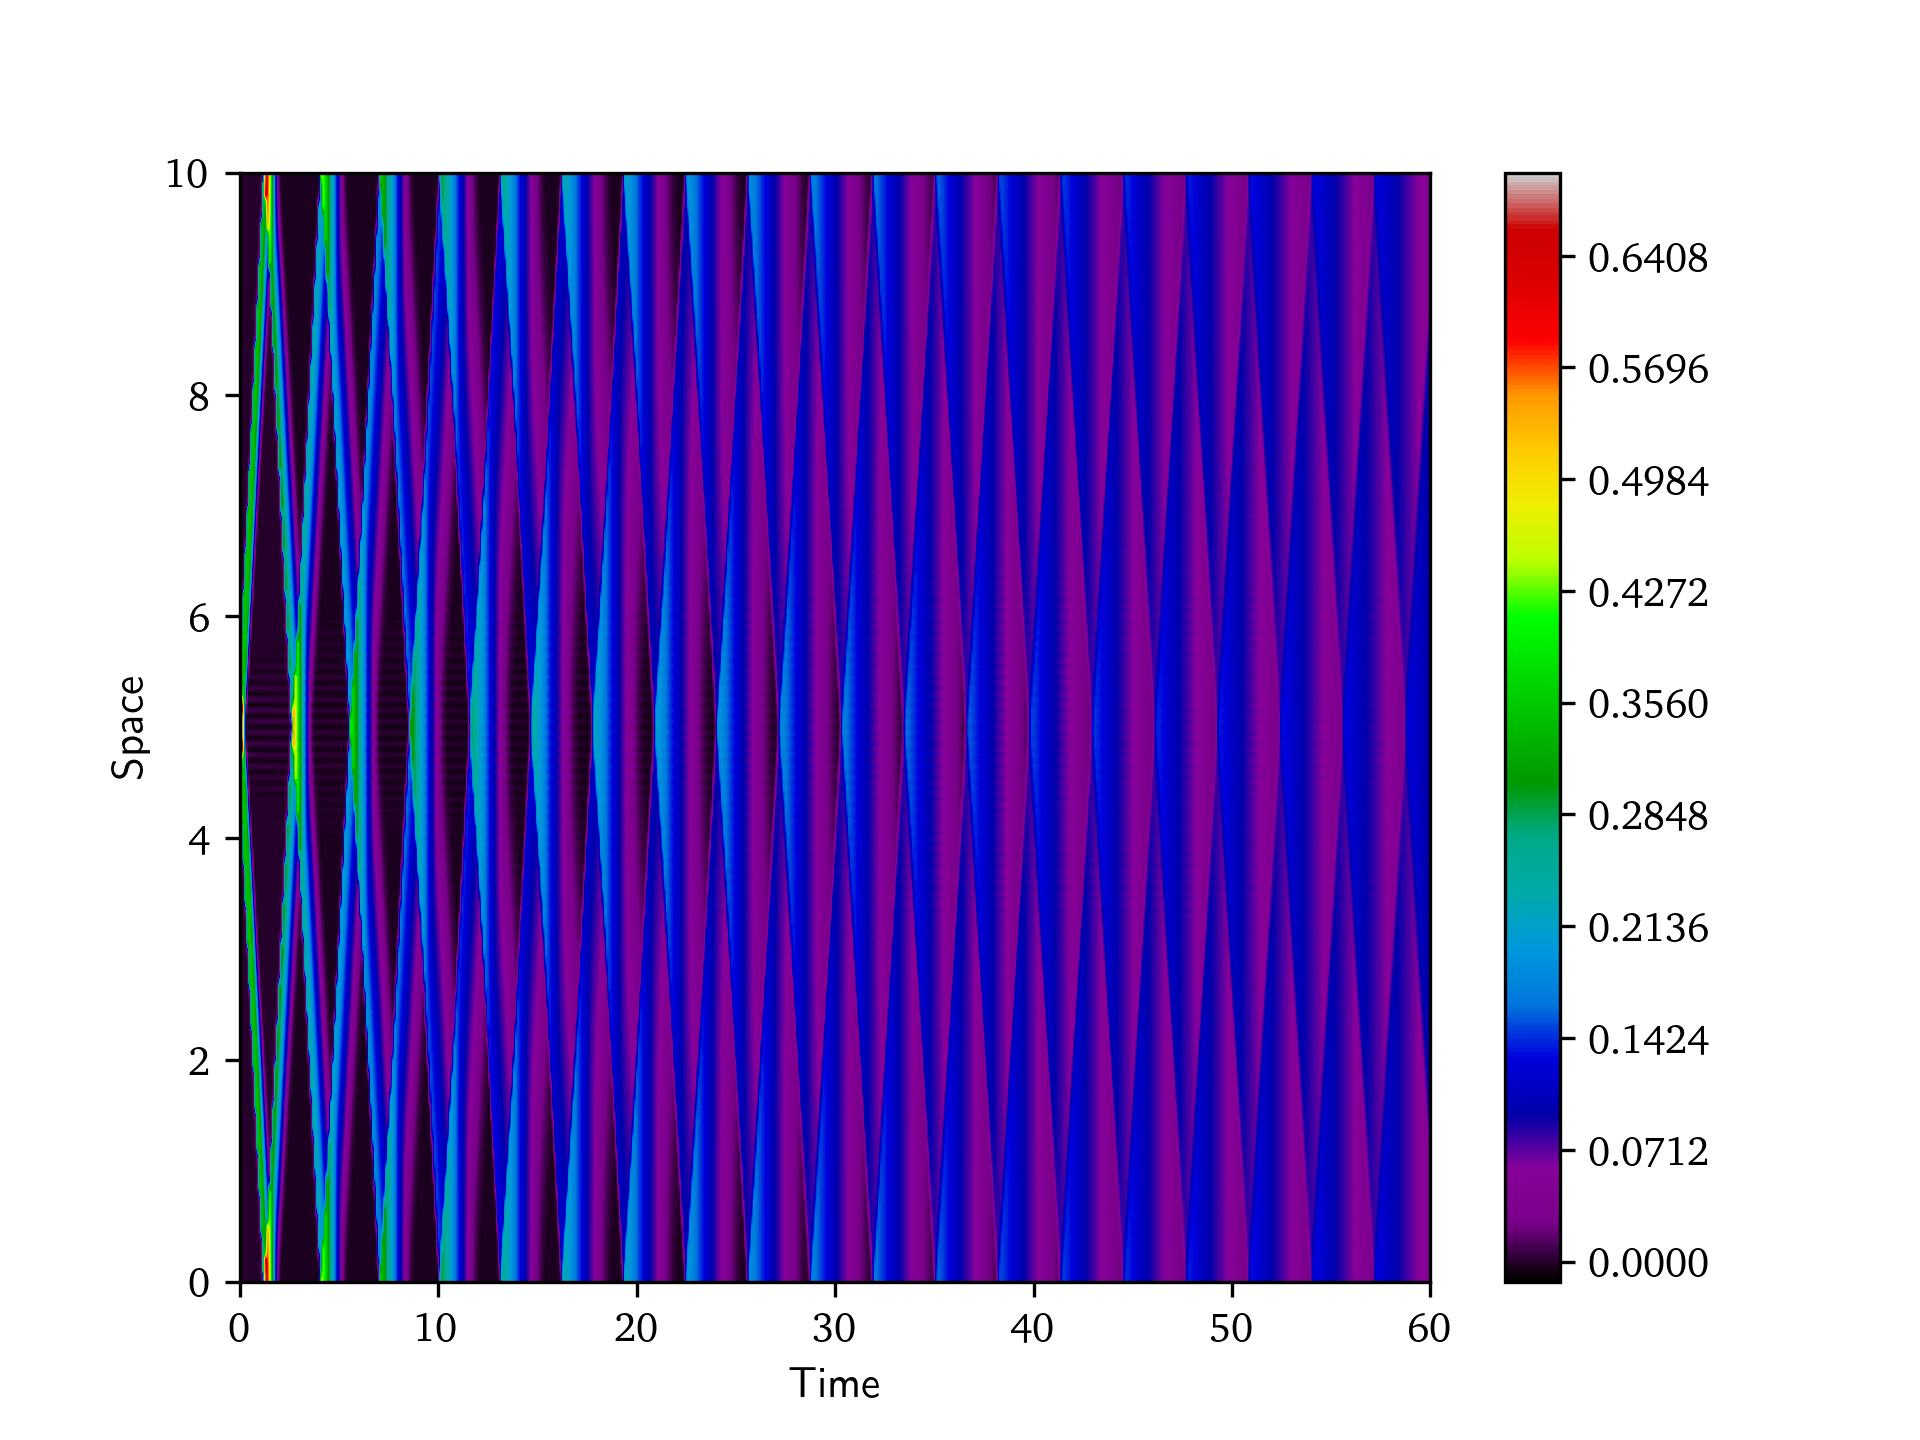
\includegraphics[scale=0.85]{pics_2d/plot_G_3_10_1_0.01.png}}
\caption{График $G$ для $T = 60$ при $C = 10$, $\gamma = 1$ и~$\mu = 0.01$.}
\end{figure}


\begin{figure}[H]
\center{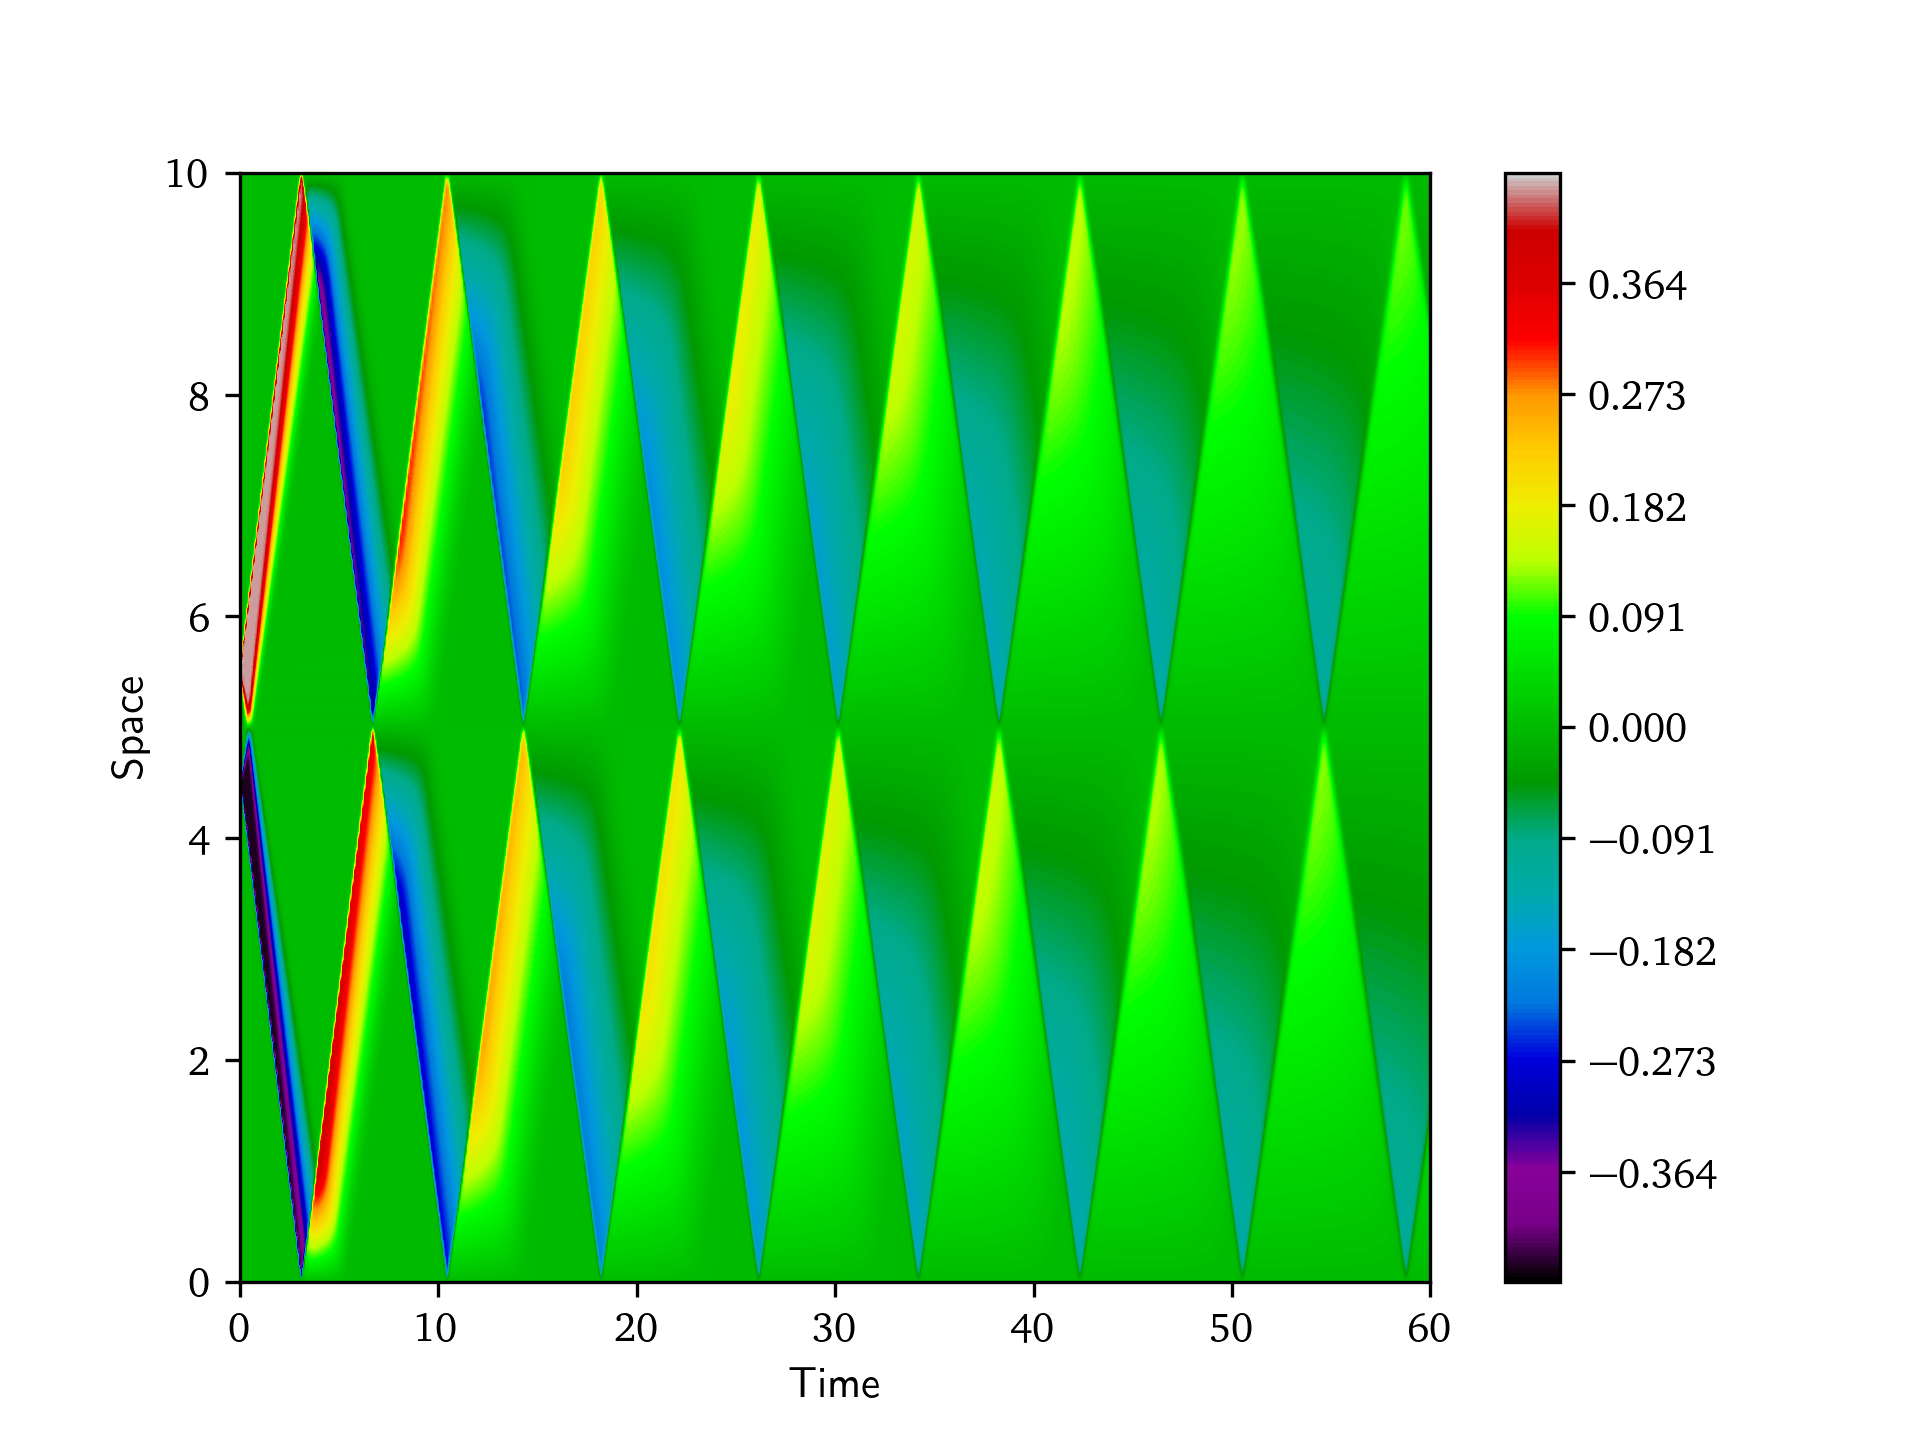
\includegraphics[scale=0.85]{pics_2d/plot_V_3_1_1.4_0.01.png}}
\caption{График $V$ для $T = 60$ при $C = 1$, $\gamma = 1.4$ и~$\mu = 0.01$.}
\end{figure}
\begin{figure}[H]
\center{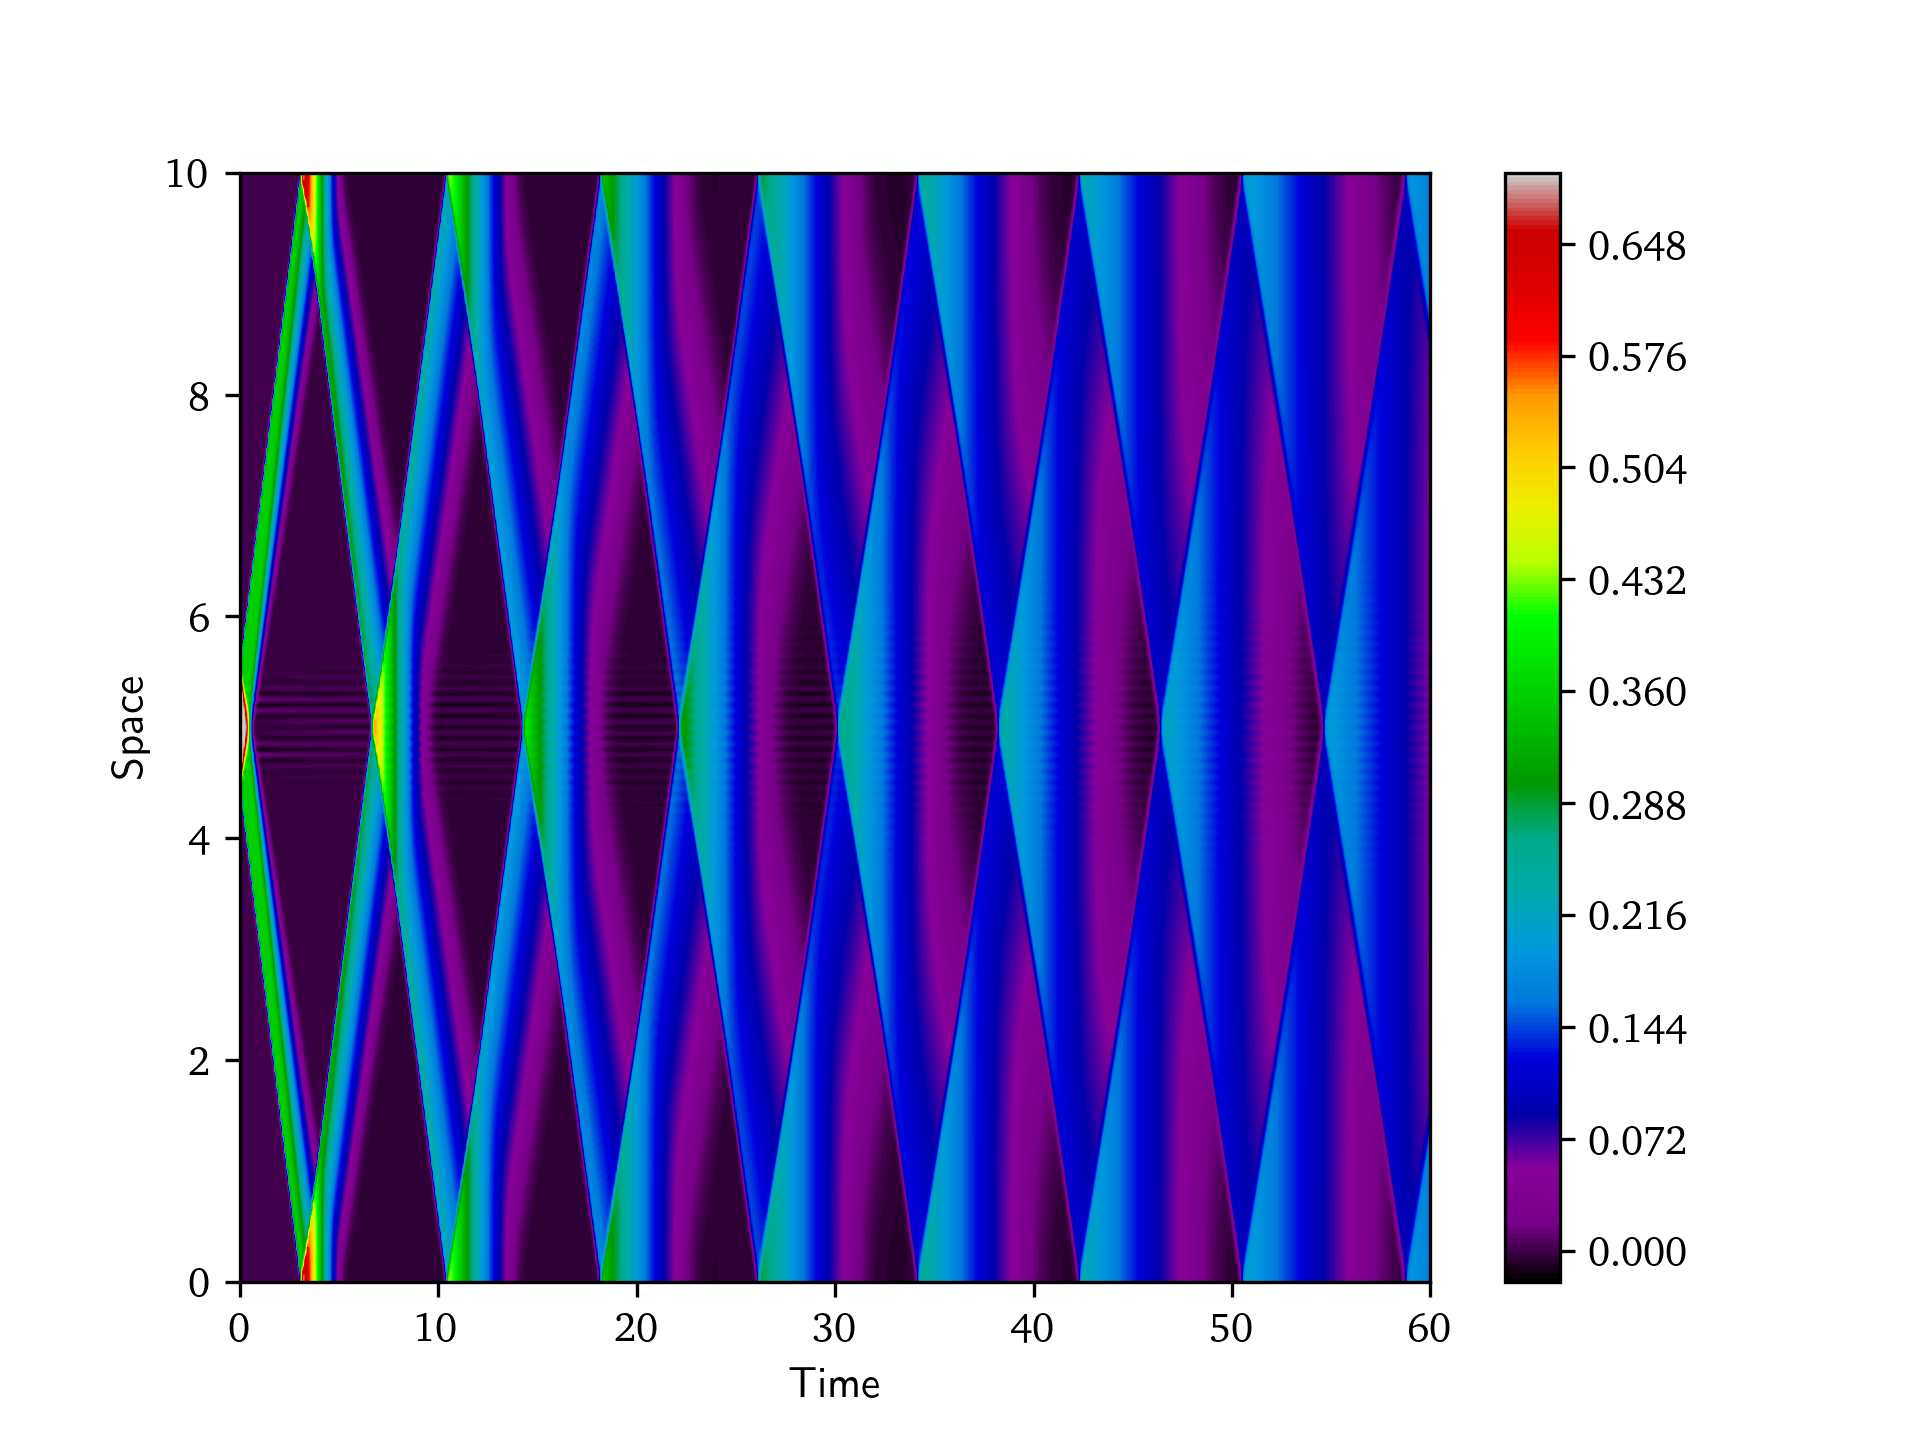
\includegraphics[scale=0.85]{pics_2d/plot_G_3_1_1.4_0.01.png}}
\caption{График $G$ для $T = 60$ при $C = 1$, $\gamma = 1.4$ и~$\mu = 0.01$.}
\end{figure}
